\chapter{Programmable Computer Networks}\label{sec:ch-networks}\label{chap:nets}
Computer networks serve the important function of allowing any two machines to communicate with one another, typically via individual messages known as packets (i.e., a packet-switched network).
Naturally, reality is much more complex than this broad statement would otherwise let on; the local routing fabric in a modern network comprises specialised (though commonplace) hardware for correctly routing these packets through arbitrary topologies of links and switches at ever-increasing data rates.
This grows more complicated still when we consider the task of \emph{inter}networking between such networks, where we must route packets on higher-level logically structured addresses between different domains of control according to fairly complex policies and relationships.
At the inception of these technologies, computer scientists of the day wisely decided that the sole duty of the network itself should be the correct routing of individual packets.
Their view was that application-level logic should be executed solely at endpoint machines; their definition extended, of course, to even include desirable (and some would say indispensable) transport-level properties such as error checking and stream reliability.
This is known as the \emph{end-to-end principle}~\parencite{DBLP:journals/tocs/SaltzerRC84}.
This position arose partly due to the logical complexity of all the tasks pushed onto the network at this time, as well as the need to ensure optimal forwarding performance while microprocessors were still relatively nascent, but was instrumental in ensuring that the network itself remained \emph{extensible}.
A consistent, pared down feature set was ensured while offering a good degree of freedom for the development and deployment of higher-level protocols.

Decades have passed since then, and to a large extent the zeitgeist has shifted on just how capable our networks should be---in both the research community and operators of large-scale networks.
Consider the case where an operator has a fully converged network built entirely on fixed-function hardware, but wishes to use some program to inspect the behaviour, state, and characteristics of some flow between two local machines.
The problem is that these devices offer no means of modifying or influencing routing state, being highly-optimised switching devices that understand a selection of routing algorithms built into their internal circuitry.
For the longest time, altering the network's routing behaviour in this instance---even for a single override---required not only physically altering and rewiring the network, but also would require additional hardware.
\gls{acr:sdn} was a key development in enabling this fine-grained routing over traffic at various layers in the protocol stack, allowing operators to offer per-flow or per-class routing for improved performance---\gls{acr:te}---or even application-aware load balancers at the switch level.
Initial forays into \gls{acr:sdn} were built on exploiting a separate \emph{control plane} to install \glspl{acr:mat} and rules on target switches---mapping fields of predefined protocols to predefined actions---leaving truly complex decisions to one or more controller machines.
These developments have been pushed even further as the runtime capabilities of supporting devices have evolved into what we might now consider truly \glsxtrfullpl{acr:pdp}.
A wide variety of \gls{acr:asic}-based switches, SmartNICs, and other accelerators now offer an environment for expressing and executing truly arbitrary network logic, protocol parsers, and action definitions.

Despite all this, our general-purpose Internet remains much the same from an endpoint perspective---performance and reliability improvements aside.
Yet this increase in capabilities has revealed new strands of research in more specialised networks such as data centres, where in-controller processing would have allowed the network fabric to cooperate with its hosted applications but presented an obvious computational bottleneck.
\emph{In-network compute} is enabled by such bespoke routing environments when combined with the above advances in programmability, and is founded on the growing idea that in-path network elements such as switches, \glspl{acr:nic}, and middleboxes can (and should) host complex logic to accelerate applications, participate in flow control, or to aid in network management.
%In this field
%
%?? Talk about application benefits.
%?? In-network compute.
%
%Of course, over the last 
%?? Levels of engineering work at many levels of abstraction which interlink, interlock, and depend on one another
%
%What we have now are a wide variety of ways to run programs of varying levels of complexity at ?? many levels of the stack ?? to aid application and networkr performance

This chapter begins by motivating and describing initial attempts at dataplane programmability in the '90s (primarily \emph{active networking}), how control-plane programmability and \gls{acr:sdn} arose in their wake, and the reasons behind these movements' respective failures and successes (\cref{sec:from-fixed-function-to-fully-programmable}).
\Cref{sec:modern-pdps} introduces modern, programmable dataplanes by tracing efforts parallel to the development of \gls{acr:sdn} for improving the performance of host-based packet processing, such as \glspl{acr:vnf}, before leading into the emergence of specialised \gls{acr:pdp} hardware from legacy \gls{acr:sdn} and \glspl{acr:npu}.
This is followed by commentary on the ways that the original active networking movement differs from modern \glspl{acr:pdp} (and context behind the latter's successful adoption), as well as a selection of open challenges and proposals in \gls{acr:pdp} programming languages and hardware designs.
\Cref{sec:offloading-and-in-network-compute} then explains the rationale behind \emph{offloading} service logic to \gls{acr:pdp} hardware and into host network stacks, while describing recent research on using these capabilities to automatically accelerate existing dataplane programs.
Finally, to further motivate in-network compute I describe point solutions which take advantage of the execution environment and more granular view of network data to improve measurement and operation (\cref{sec:in-network-compute-use-cases}).
%Finally, \cref{sec:problems-in-modern-networks} provides some literature on volumetric \gls{acr:ddos} attacks (and defences against them) as necessary background for \cref{chap:ddos-rl}.

\section{From fixed-function to software-defined}\label{sec:from-fixed-function-to-fully-programmable}
%?? What are networks?
%
%?? Possibly discuss the internet
%
%?? Lead in from ARPAnet et al. (2 paras). Scientific comms -> general use,
%
%The intro of choice~\parencite{DBLP:journals/ccr/FeamsterRZ14}
%
%?? interconnection physical and reconfig are main challenges that made SDN look attractive, reasonable?

%Control plane programmability: routing etc? Dataplane programmability: per-packet computations.
%?? focus on programmable \emph{dataplane} rather than control plane

Initially, network fabrics were \emph{fixed-function}, supporting only the routing algorithms provided by permanent \glspl{acr:asic} integrated with their silicon, and offering transit only for protocols considered at their construction.
However, from the Internet's origin as ARPAnet through today, programmability of networks has increased over time to simplify the management, use, and adaptability of network infrastructure~\parencite{DBLP:journals/ccr/FeamsterRZ14}.
Programmability in computer networks tends to be categorised into two distinct forms.
\emph{Control plane} programmability focuses on the routing of packets, making it easier to alter, update, and tailor the forwarding behaviour of a network at run time, and at many levels of granularity.
%?? Programming the \gls{acr:fib}/\gls{acr:rib}
\emph{Dataplane} programmability focusses instead on introducing additional logic into the network to be executed by the forwarding elements such as routers---stateless or stateful transformations of packet streams, traffic measurement, and so on.
We examine first \emph{active networks}, one of the earliest movements to enable network packet processing at the infrastructure level.
%There is, of course, vast scope for their interaction. ?? describe

\subsection{Active networking}\label{sec:active-networking}
In response to the expanding scale and widespread reach of the Internet (and computer networks in general), researchers in the early-to-mid '90s increasingly desired the tools to extend, innovate, and research routing and transport protocols.
To maintain and safeguard interoperability over the Internet, the \gls{acr:ietf} formed to maintain and oversee the development of Internet protocols for all levels of the networking stack.
The weight of full \gls{acr:ietf} standardisation was seen by many researchers of the period as a lengthy process, which they believed to be the cause of \emph{network ossification}---the Internet becoming inflexible to the design and deployment of new protocols.\sidenote{Authors of this period might be horrified to discover that the \gls{acr:ietf}'s median time to standard publication has more than doubled since 2000~\parencite{DBLP:conf/imc/McQuistinKKPTPH21}. This is not, however, what we understand as ossification in today's Internet, which I'll discuss shortly.}

\emph{Active networking} was researchers' response: a family of clean-slate proposals built around enabling switches to perform arbitrary computations on carried packets, and for the network to share resources such as compute and memory with users and applications~\parencite{DBLP:journals/ccr/TennenhouseW96,DBLP:journals/ccr/Calvert06}.
This is a more communistic, cooperative view of the role of the network---that it should provide and manage advanced services as a sort of common good beyond raw forwarding capacity and functionality, more than simply `best-effort'.
%Shared resources, expectation of the network to `do something'.
This would enable not only new protocols empowered by the cooperation of the routing fabric, its proponents argued, but would also simplify network management and measurement; it was in no uncertain terms a radical departure for its time, standing in stark opposition to the simplicity demanded by the end-to-end protocol.
Active networks planned to enable caching and \gls{acr:cdn}-like behaviour, stream compression, network management, and enhanced telemetry.
Similarly, they could transparently improve data transfer with in-path compression or error correction via \emph{protocol boosters}~\parencite{DBLP:journals/jsac/FeldmeierMSBMR98}.

Surveys of today divide the ideas of this movement into two main streams of research~\parencite{DBLP:journals/ccr/FeamsterRZ14}:
\begin{description}
	\item[Capsules,] which consisted of compact programs bundled with network packets; either at a per-packet level, or installed on a per-flow basis during the handshake process.
	\item[Programmable switches,] which allowed arbitrary programs to be installed by system administrators to their own infrastructure for dataplane processing.
\end{description}
These are two key tools rather than opposing schools---and works we'll examine from the tail end of the \emph{active networks} movement feature a high degree of interplay between both ideas.
It must be said that in the absence of specialist supporting hardware, the vast majority of works in this field relied entirely upon execution of high-level code via commodity host machines.
\gls{acr:udp} tunnelling and overlay networks like \emph{PlanetLab}\sidenote{PlanetLab also had a wider effect on distributed systems research. Sadly, it was shutdown in May of 2020~\parencite{planetlab-rip}.}~\parencite{DBLP:journals/ccr/ChunCRBPWB03} were necessary to do so; the former modelling a cooperative multi-\gls{acr:as} Internet in a testbed setting, and the latter providing hosts with \gls{acr:cpu} and memory slices across the world in a ticketed, quid-pro-quo manner.

\paragraph{Innovations in capsules}
\emph{ANTS}~\parencite{ANTS,DBLP:conf/dance/Wetherall02} captured the stereotypical active networking idea of `arbitrary user programs' carried by each packet.
A capsule contains one or more program IDs in each header's packet, to be inspected by an ANTS runtime at on-path active nodes.
Capsules include dataplane programming and routing logic, kept immutable between flows.
An active node checks its local cache for program code matching a capsule's IDs, which may be pre-installed by an administrator (out-of-band); on a cache miss, the code is requested from the last active node (in-band).
Programs for a given ID are verified and signed externally by some trusted organisation e.g., the \gls{acr:ietf}, but their use is still controlled by \emph{the user or endpoint application}.
%?? in-band and out-of-band installation: pre-install or request prog from prior hop on miss.
ANTS relied on the transfer of Java code: extensions such as \emph{PAN}~\parencite{PAN-activenet} investigated the use of raw unsafe x86 assembly for performant in-kernel use.

\emph{Smart packets}~\parencite{DBLP:journals/tocs/SchwartzJSZRP00} examined dataplane programming from the perspective of measurement and control.
Intended as a means for management centres to install packet programs on managed nodes, one or more initialisation packets would be sent across the network between a source and destination---each containing a single complete program and all relevant authentication certificates.
Any nodes along the path---including endpoints---would be free to install or pass on logic as required.
Programs were limited, stateless, compact programs executed in a \gls{acr:vm} for all carried packets, with dedicated intrinsics for accessing state from the \gls{acr:mib}; packets could trigger \gls{acr:mib} events, or modify a packet to include per-path telemetry supporting passive and active measurement use cases.
Hosts and switches were expected to enforce limits on execution time and dynamic memory use to keep the scheme feasible at scale.

\emph{NetScript}~\parencite{DBLP:journals/jsac/SilvaYF01} allowed for the definition of active network programs as a dynamic (i.e., potentially branching) dataflow graph of smaller programs---\emph{boxes}.
Such boxes may be recursively defined.
Crucially, its main advantage over the similar \emph{Click}~\parencite{DBLP:conf/sosp/MorrisKJK99} is that any box can be a remote node (another machine, or a specialised hardware/\gls{acr:asic} implementation), which makes this a remarkably prescient combination of control plane and dataplane programmability.
Dataplane program definition and selection is left entirely to network operators in this abstraction, rather than allowing tenants' code.

\paragraph{Switch programmability}
Though conceptually purer uses of programmable switches are rare in this movement, their use is often implicitly assumed to be necessary in any real, performant active network.
The \emph{SwitchWare} project~\parencite{DBLP:journals/network/AlexanderAHKKMG98}, while very much a capsule-based proposal, primarily suggested a base of \emph{SANE}-backed switches~\parencite{DBLP:journals/network/AlexanderAKS98} which would implement a fixed, performant set of `active extensions' analogous to \gls{acr:os} syscalls.
Ahead-of-time fixed subprograms like these were key here to achieve performance and security---mainly by limiting capsule program capabilities and allowing delegation to \gls{acr:asic} accelerated operations in performance-critical scenarios.

From a more practical perspective, \Textcite{DBLP:journals/jsac/WolfT01} examine the design requirements of a programmable switch in contrast with emerging \glspl{acr:npu} of the time.
They propose a \gls{acr:soc} design built around a large array of general-purpose \gls{acr:risc} \glspl{acr:cpu}, each having their own cache and memory.
A first stage \gls{acr:asic} would route packets to an output port over a shared interconnect, where these \glspl{acr:cpu} would either count as their own port or be attached to a physical egress and conditionally used.\sidenote{Curiously, this design more closely matches modern SmartNIC devices, while today's programmable switches favour \gls{acr:asic} designs. We'll return to this point in \cref{sec:pdp-specd-hw}.}
The use of complete \gls{acr:risc} \glspl{acr:cpu} is quite deliberate: early \glspl{acr:npu} such as the Intel IXP1200~\parencite{intel-ixp} and Lucent's Fast Packet Processor~\parencite{lucent-fpp} had unusual instruction sets suited to stateless processing of headers~\parencite{DBLP:conf/pldi/GeorgeB03}, limiting their general expressiveness.
A fuller \gls{acr:isa} was recognised as being necessary for more capable, general, useful, and stateful dataplane programming; particularly of the kind envisioned by active networking.

%, which is where perf-router cite succeeds. ?? stateless etc.

%?? mention smartpackets's exec model here.

Returning to \emph{smart packets}, we see a similarly earnest attempt to reconcile capsule networks with a reasonable programming framework (as opposed to its peers' focus on high-level languages).
Aiming to be more amenable to switches they propose \emph{Spanner}, a compact \gls{acr:cisc} assembly language for a stack-based \gls{acr:vm} with primitives to access the \gls{acr:mib}, compiled to from their own higher-level language.
Spanner was designed to be reasonably implemented on hosts and routers, but explicitly trades performance for compactness; focussing on small, self-contained, secure programs.\sidenote{This shares many conceptual similarities to \gls{acr:ebpf}, a \gls{acr:risc} register machine, which now plays a key role in network compute offload and \gls{acr:os} kernel extensibility. I introduce \gls{acr:ebpf} in detail during \cref{sec:host-offloading-technologies}. The \gls{acr:vm} abstraction, using intrinsics and maps to communicate with the environment, ensures security while the language's simplicity allows implementation in the network fabric.}
The executing switch or host enforces memory and execution limits at runtime, but single-packet $\mathcal{O}(\text{\qty{1}{\kibi\byte}})$ programs simplify deployment logic.
Naturally, this excludes stateful boosters of the type we've examined, but is well-suited to the measurement and management use cases its authors intended.
%?? HLL -> \gls{acr:cisc} Assembly for stack-based \gls{acr:vm}\sidenote{}, with primitives to access \gls{acr:mib}. Focus: small, self-contained, stateless secure.

\paragraph{Failings and drawbacks}
Sadly, the active networking paradigm failed to properly fledge, at least in its first iteration.
It might be argued that the `communistic' network view played a key part in this downfall---that the tangled web of \glspl{acr:as} between any two nodes should freely offer compute resources to the benefit hosts.
This comes down to a simple question of economics: who pays whom for providing these services?
It's easy to reason about this in campus or internal networks (the organisation provides active capabilities as part of its own remit), or if we require that only our \gls{acr:isp} offers these capabilities (hosts pay for them explicitly).
Extending this notion to the wider Internet becomes more challenging.
Assigning responsibility for administrative, technical, and security issues among all the organisations between two endpoints is a daunting prospect, to say the least.
When modifying packets in a protocol booster-like model, it becomes difficult to communicate where boundaries of support start and end to enable truly transparent behaviour.
In a setup like the PlanetLab overlay network the incentives for providing these capabilities in such a distributed way are obvious: all the users are researchers in need of distributed compute.
Each benefits from donating compute and network slices in their own infrastructure to receive resources in kind.

The problem here is also one of aggregation.
At the Internet core such as in \glspl{acr:ixp}, transit bandwidth demands are the sum of all connected \glspl{acr:as}, amplifying compute demands and scale concerns.
From another angle, suppose that all functions benefit the network \emph{and} hosts alike, as in the case of an in-band \gls{acr:tcp} compressor.
Here, files can be transmitted between end hosts quicker \emph{and} the bandwidth impact on the switching fabric is reduced.
If hosts benefit and have the resources to implement this functionality it is inevitable that at some point they will do so (pushing logic to the network edge), at which point network operators are able to put their own resources into faster or higher-capacity passive infrastructure with a vastly reduced attack surface compared to an active solution. 
On the upside, this also preserves the end-to-end principle.

% is part of its downfall administrative, tech, security issues etc. Even though some use cases would have benefited admins (i.e. compression to expand capacity).
%?? Obvious in PlanetLab: incentives are all users are researchers!
%?? Lots of economic drivers: who pays whom for providing these services? Why not just push this logic to hosts (preserving end-to-end) if the logic (i.e. compression) benefits the network AND hosts too?

%?? More issues? complexity, where boundaries of support start and end (and how to communicate them) (for instance, in protocol boosters).
%?? Flow migration and redundant failover, and path aggregation far harder?
%?? In ANTS, implications for flow buffering on prog miss.

Active network capabilities do in many senses \emph{limit} how networks can benefit their users (or at least make some innovations substantially harder).
Consider flow migration, potentially as part of a wider \gls{acr:te} strategy, or path aggregation to increase bisectional bandwidth or provide redundancy to protect from link failures.
Administrators must not only handle routing and design of such capabilities, but they must also ensure that active network programs on any flow's path are mirrored or migrated to the new path.
In the event of a complete or partial node failure, this may not be trivially possible.
Even when retrieving programs from the last hop, failover may be needed for a live high-bandwidth flow, requiring costly per-flow buffering at a node until capsule program setup is complete.

The capabilities of programmable switch hardware were, to some extent, overshadowed by the community's focus on the more intoxicating idea of capsule networking.
Naturally, the overwhelming majority of these platforms were prototyped on host machines, which limited forwarding and processing performance far below that of even early Ethernet.
The repeated emphasis on high-level prototypes reduced the focus on the sorts of low-level, capable languages a performant system would require---proposals were instead marred by in-vogue high-level \gls{acr:vm}-based languages such as Java and Caml, which did their credibility little good.
This likely also added to industry scepticism---one gets the sense of a paradigm driven by research trends instead of limiting its own boundaries to produce something truly capable and scalable.

\subsection{Software-defined networking}
In parallel, a good many researchers saw a need to innovate (and fight stagnation in) the space of what we now understand as control plane programmability: the ability to deploy and develop new routing protocols, provide bespoke routing for individual packets, flows and applications, and to adapt to changes in the network itself.
While likely starting out from the same perspective as active networking---enabling new capabilities and development, and network evolution---as years have gone by greater network capacities, usage demands and a need for far greater reliability have introduced challenges manyfold.
Greater capacities, particularly in bisection bandwidth, typically mean more routers and switches for network admins to manage, but also in terms of additional cabling for link redundancy and aggregation---neither of which play well with older spanning tree protocols.
\glsxtrfull{acr:te}---making effective use of this capacity and providing different traffic classes with optimal forwarding---has similarly become more and more important over time.
The problem is that classical routing protocols such as \gls{acr:ospf} and \gls{acr:rip} are designed for distributed autonomy, offering no support for direct routing rule insertion by administrators.
Early \gls{acr:te} approaches were thus built on a shaky foundation of hacks and tricks, exploiting routing protocol behaviour to achieve the desired high-level outcomes~\parencite{DBLP:journals/ccr/FeamsterRZ14}.
Naturally, such workarounds become untenable and impossible to reason about at scale---particularly as failures and misconfigurations creep in and become harder to find and diagnose.
Effective though these early methods were, they remained hamstrung by the tightly coupled control and data planes of the network hardware of that era.
The reality and urgency of this problem space has led to the true separation of forwarding elements (the dataplane) from the logical control elements which inform and orchestrate their routing behaviour (the control plane).
With the advent of the control plane, \glsxtrfull{acr:sdn} arose too---the use of arbitrary machines and logic to define the forwarding behaviour of each and every network element~\parencite{DBLP:journals/comsur/NunesMNOT14,DBLP:journals/ccr/FeamsterRZ14}.
As we shall discuss, this has brought forth a well-developed and successful bevy of innovations in network control and design.

\paragraph{Development of the control plane}
This line of work began in earnest with the \emph{open signalling} movement~\parencite{DBLP:journals/ccr/CampbellKMV99} in \gls{acr:atm} networks, circa 1995.
Open signalling aimed to standardise the \glspl{acr:api} and protocols for passing routing data to its relevant handler (and rules to line-cards) in an era where these elements were still tightly bonded in commercial routing hardware.
\emph{Tempest}~\parencite{DBLP:journals/network/MerweRLC98} marked its zenith, using these capabilities in tandem with specific functions of these now-obsolete \gls{acr:atm} networks to define a `network control architecture' which would oversee correct forwarding policies and resource allocation.
Its primary focus, however, was in providing independent virtual network slices---\emph{switchlets}---to users of multi-tenant networks on demand, allowing these users to pass in their own control programs written for host execution in Java, for instance.
Control plane traffic from control elements to the dataplane was carried \emph{in-band} at this time (i.e., using the same fabric as tenants' datagrams).

%?? What do I want to cover? first: separation of ctl plane, OF and Net OSes (ONOS, OpenDaylight, ...), then bring around to vNFs etc
%
%Tempest~\parencite{DBLP:journals/network/MerweRLC98} for ATM networks, built on principle of \emph{open signalling}~\parencite{DBLP:journals/ccr/CampbellKMV99} (in ATM) from 1995. IP/Ethernet networks still `bonded' FEs and CEs in routing design.
%
%?? Greater capacity and use forced focus on \gls{acr:te}, which was onerous and required insane workarounds w/ fixed-fn hardware~\parencite{DBLP:journals/ccr/FeamsterRZ14}

These ideas were refined into a standard for hardware elements on a shared bus via \emph{ForCES}~\parencite{rfc3746}; stripped, of course, of the more visionary aspects such as network slicing, arbitrary control code, and wider resource management.
Primarily, this was focussed on registration of control plane elements, including key provisions for extensibility and discoverability to announce additional protocols and offer redundancy.
The move to physically remote control elements was proposed by \emph{SoftRouter}~\parencite{lakshman2004the}, such that forwarding and control elements would communicate with one another in-band over the same network they define (after a simple spanning-tree bootstrap phase) using custom discoverability protocols.
This allowed its authors to experiment with reducing the number of control elements in a network, from which they observed faster convergence of protocols such as \gls{acr:ospf}.
Hardware capabilities did not at this point allow this level of control, and as such host-based kernel dataplane routers like \emph{XORP}~\parencite{DBLP:journals/ccr/HandleyHK03} and simulators such as \emph{ns}~\parencite{Bajaj99improvingsimulation} reigned in research at this time.

Most of the above work focusses on the \emph{intra}-domain case---routing \emph{within} an \gls{acr:as}.
\emph{RCP}~\parencite{DBLP:conf/nsdi/CaesarCFRSM05,10.1145/1016707.1016709} was instead motivated by how \emph{inter}-domain routing \emph{between} \glspl{acr:as} might benefit from the sorts of centralised control we now associate with \gls{acr:sdn}.
The problem in this instance is that edge routers must understand and implement \gls{acr:bgp}, each having their own arcane policies to achieve the intended network behaviour with respect to quirks of the protocol, their own hardware, and the routes forwarded by neighbouring \glspl{acr:as}.
Their solution was to centralise this logic into one (or a few) host machines, providing a drop-in solution which could act on \emph{all} gathered \gls{acr:bgp} information to produce optimal decisions with better scaling characteristics, reduce administrative overhead and fragility, and which opened the door to later extension if neighbour \glspl{acr:as} also deployed RCP.

With the growing need for \gls{acr:te} and \gls{acr:to} at various layers of the Internet infrastructure, we begin to see a drive for wider coordination in the intra-domain case.
\emph{PCE}~\parencite{rfc4655} is one of the first serious attempts to formalise a network architecture where the control plane can calculate and install bespoke \emph{paths} at the flow level, given any set of constraints.
Naturally, this requires far greater coordination of the individual forwarding behaviour of switches, preferably combined with \gls{acr:mpls}.
\emph{Ethane}~\parencite{DBLP:conf/sigcomm/CasadoFPLMS07} pushed this notion of complete network control further; a dedicated controller overseeing the forwarding rules and paths installed at an entire network of `dumb' switches, containing \emph{only} an action table of \emph{exact} matches.
Their goal was not one of performant \gls{acr:te}, however, but of policy---complete control over interactions between named entities and their classes, with all flow misses being directed to the controller.\sidenote{It's worth noting that this proposal was intended only for campus networks, hence its obvious scalability limits don't bite quite as badly as they might in, say, an \gls{acr:ixp} or data centre. In particular, it must upcall to the controller for every new address, and maintain an exact match rule for every live flow due to the lack of longest-prefix matches.}
The controller then authenticates, authorises and orchestrates all host-to-host connections according to a given policy.

The arrival of \emph{OpenFlow}~\parencite{DBLP:journals/ccr/McKeownABPPRST08} marked a watershed moment in \gls{acr:sdn}, iterating on Ethane's key ideas to remove notions of authentication, focussing more on the network itself.
Motivated to lower the barrier of entry for experimentation and research in the routing domain,\sidenote{In-text, this is again referred to as ossification: here arising from the closed nature of routing hardware coupled with the performance needs of realistic traffic.} OpenFlow decided to change tack compared with XORP and its contemporaries by targeting real hardware (and by tailoring its design to capabilities of commodity devices of the day).
OpenFlow kept Ethane's \gls{acr:mat} abstraction, as switches of that era stored flow tables internally, and required support for few actions: forward packets on a port, drop packets, encapsulate and send a packet to a designated controller, or defer to the switch's underlying forwarding logic.
Each OpenFlow switch then maintains a dedicated, secure connection to at least one controller, though may receive rules from any number of them.
This was set apart from its earlier competitors and progenitors by its drive for easy compatibility with commodity hardware, for instance by providing their own open source OpenWRT firmware.
What it then codified was an open, consistent manner for software to configure the routing behaviour of real hardware at the whim of operators, going so far as to suggest that high-performance dataplane programmability might be enabled via steering to NetFPGA devices elsewhere in the network---eliminating virtualisation.
The supported capabilities and reach have expanded somewhat since its initial, academic, limited introduction.
Indeed, while we now understand that OpenFlow has incredible value in the operation and management of large networks, the vision embodied by the original work is in fact much closer to the `switchlet' model of Tempest where individuals request transit for traffic between their machines, carrying their own experimental protocols or enacting novel policies.
The specification has thus evolved over time to include features more useful and tailored to complex networks and costlier hardware: conditional support for more expressive actions and matching capabilities, including additional tables, groups, egress processing, and packet header modification~\parencite{openflow-1-5}.

\paragraph{An ongoing legacy}
The remarkable thing about the field of \gls{acr:sdn}, particularly compared to active networks, is that it's still here.
Moreso than that, it plays a large role in modern networks of hypergiant scale. 
We'll discuss a case study shortly.
%Why has this worked so much more effectively?
Why has control plane programmability proven to be so much more effective and attractive to operators in practice?

Principally, it is because control plane programming is easier to get right---in the sense of processing speed and volume.
Routing information, link states, and topology changes collectively arrive at a far slower rate than packets, or even simply carried flows.
An OpenFlow controller is under no obligation or need to, say, react to millions of routing changes per second while adding only microseconds of latency, because the routing \emph{environment} varies at a rate which is well suited to the processing capabilities of commodity hosts.

Secondly, the wide reach of open-source software for developing, deploying, and testing \gls{acr:sdn} concepts and ideas has helped these ideas gain traction in both the research community and in real-world deployment.
Network \glspl{acr:os} and controllers such as  \emph{NOX}~\parencite{DBLP:journals/ccr/GudeKPPCMS08}, \emph{Onix}~\parencite{DBLP:conf/osdi/KoponenCGSPZRIIHS10}, \emph{ONOS}~\parencite{onos}, \emph{OpenDaylight}~\parencite{opendaylight}, and \emph{Ryu}~\parencite{ryu} provide moderately easy interfaces for programmers to implement their own controllers.
Network emulators such as \emph{mininet}~\parencite{DBLP:conf/hotnets/LantzHM10} allow researchers to define and operate virtual networks built entirely of OpenFlow-capable switches on their own machines using host programs and standard sockets to generate and use carried traffic, enabling easy prototyping.
High-performance software switches such as \gls{acr:ovs}~\parencite{DBLP:conf/nsdi/PfaffPKJZRGWSSA15} offer first-class support for OpenFlow and no small number of extensions, and are instrumental in data centre virtualisation~\parencite{DBLP:conf/sigcomm/TuWAP21}.

%?? Why the success? iterative, built on existing tech with an easier-to-use interface etc.
Finally, the movement capitalised on \emph{existing hardware} and its own capabilities, rather than calling for a radical wave of enhancements or brand new, expensive capabilities.
Providing a higher-level abstraction to manage the infrastructure which networks already contained ensured the adoption and current success of \gls{acr:sdn}.

%?? A survey to mine for stuff~\parencite{DBLP:journals/comsur/NunesMNOT14}

One well-documented, well-published, and arguably ongoing case study of this paradigm in action at scale is the wave of high-impact papers produced by Google.
Google's \emph{Jupiter} data centre network design~\parencite{DBLP:conf/sigcomm/SinghOAAABBDFGK15} was developed concurrently with most of the works outlined above, where these techniques have been instrumental in managing the explosive uptick in switch hardware demanded by their larger Clos topologies.\sidenote{Particular issues demanding custom routing and administration include the vast amount of multipath complexity at this scale, heavy per-link state, and potential performance gains from network homogeneity that general-purpose routing algorithms might fail to capture.}
Additionally, \gls{acr:sdn} techniques have helped to manage phased integration of this new network.
In \gls{acr:wan} topologies, \emph{B4}~\parencite{DBLP:conf/sigcomm/JainKMOPSVWZZZHSV13} has made direct use of OpenFlow for \gls{acr:te}, to maximise link utilisation and offer resilience (aided by the fact that Google own the \gls{acr:wan} endpoints).
The architecture evolved fairly cleanly over the following 5 years, coping with \qty{100}{\times} bandwidth increases and more stringent reliability bounds~\parencite{DBLP:conf/sigcomm/HongMAZABBJKLMP18}.
\emph{Espresso}~\parencite{DBLP:conf/sigcomm/YapMRPHBHKNJLRR17} extends this to inter-domain peering arrangements with the Internet and \gls{acr:bgp} session management, finally realising the vision of RCP 13 years on.
Nowadays, their data centre and \gls{acr:wan} networks are managed by a single higher-level microservice \gls{acr:sdn} architecture, \emph{Orion}~\parencite{DBLP:conf/nsdi/FergusonGHKMMOP21}.

\section{Modern programmable dataplanes}\label{sec:modern-pdps}
While active network research may have dried up in the last 20 years,\sidenote{Barring some very obvious throwback works such as \emph{Tiny Packet Programs}~\parencite{DBLP:conf/sigcomm/JeyakumarAGKM14}---which have directly influenced new in-network telemetry schemes like those we cover in \cref{sec:network-monitoring}.} interest in dataplane processing has remained strong.
Network operators have, in fact, always had a need for complex packet processing to measure, protect, and enhance \emph{their own} networks---rather than to provide the sort of communal good that active networks promised.
To offer some examples:
\begin{itemize}
	\item \emph{Firewalls} are a necessity for filtering unauthorised traffic at stub \glspl{acr:as}, but require line-rate lookups versus large allow- and block-lists across varied protocols. Similarly, \gls{acr:nat} boxes play an important role for \gls{acr:isp} networks.
	\item Protocol enhancements and \gls{acr:te} solutions, such as \emph{\gls{acr:wan} optimisers} and \emph{application-layer load balancers}, which need to be able to inspect and/or modify traffic based on (possibly complex) transport-layer and application-layer semantics.
	\item Security functions, such as \glspl{acr:ids} and \gls{acr:ddos} traffic scrubbing solutions. These can require complex, stateful logic (such as regular expression matching and transparent datagram reassembly) that makes them challenging to implement while maintaining high performance---particularly when we consider that the \gls{acr:ddos} use case \emph{demands} that we keep up with a high ingress traffic volume.
\end{itemize}
At scale, the performance challenges involved in per-packet and per-flow processing for these functions becomes difficult to reconcile with the performance limitations of host machines.
The obvious solution is to fall back to silicon in pursuit of performance, and as a result the market has long included so-called \emph{middleboxes}---bespoke \gls{acr:asic} devices designed to perform one or more pre-defined dataplane functions at line rate.

An obvious trade-off has been made here: runtime programmability has been sacrificed for performance.
What is less obvious is that another, hidden, cost has been introduced owing to the fallibility of engineers---our final source of network ossification.
While effective at their designed tasks, middleboxes are infamous for relying on the \emph{observed} behaviour of network traffic rather than the behaviours actually decreed in the relevant \gls{acr:ietf} standards and specifications.
As a result, they have become a barrier to the wider deployment and introduction of protocols in the Internet.
\gls{acr:sctp}~\parencite{rfc4960} is one recent example of an approved protocol whose deployment has been hobbled by the prevalence of middleboxes that expect only a limited suite of layer-4 protocols~\parencite{sctp-middlebox-bad}.
Under the same considerations, the \emph{QUIC} transport protocol~\parencite{DBLP:conf/sigcomm/LangleyRWVKZYKS17} must be tunnelled over \gls{acr:udp}, even though its Internet-wide deployment is backed by the weight of hypergiant provider Google.

%?? issues w/ their config and integration from an operational perspective
These devices also introduce operational and logistical challenges around their configuration and installation within the network.
%?? Initially, full-on rerouting.
Although \gls{acr:sdn}-based steering has to some extent obviated the need to physically rewire middleboxes' cabling when they need to be reconfigured, they do still present challenges beyond the above network fragility.
%?? Now SDN can help simplify
%?? Still issues with placement, lock-in, reconfig'ability...
Specialised middleboxes are expensive, demand rack space and introduce their own power and cooling demands, making deployment harder to scale out as network traffic demands increase.
They are failure-prone, require specialist knowledge to operate, and are vulnerable to vendor lock-in~\parencite{DBLP:conf/sigcomm/SherryHSKRS12}.
Moreover, their fixed nature makes them difficult to modify, upgrade, and fix; a sunk cost which cannot be recouped or repurposed as network function requirements change or evolve.

%?? Ossification in today's sense? Middleboxes? i.e. barrier to wider deployment even after standardisation i.e. hobbled SCTP~\parencite{rfc4960}, forced QUIC onto UDP. Also, middleboxes expensive and require work to integrate.\sidenote{Ossification causes: weight of \gls{acr:ietf}, desire for perf causing hardware impls (inflexible), over-reliance on observed behaviours of network \& protocols rather than the specs.}

The result of these drawbacks is that a constant desire has remained to introduce and capitalise on true dataplane programmability.
%?? Probably two streams: capable hardware (and its programming), and making host-based solns faster.
The pursuit of this goal can be divided quite neatly into two streams.
The first carries on from the use of virtualisation---already common in active networking research before the introduction of a true programmable dataplane fabric---towards more flexible deployment through \gls{acr:nfv} and \glspl{acr:vnf}.
The second stream instead follows from asking how we might make switching and forwarding hardware itself more programmable, keeping in mind the tight form-factor and performance bounds required of high-speed commercial network hardware.

\subsection{Virtualisation and commodity machines}
Commodity \glspl{acr:cpu} are already arbitrarily programmable, yet their dataplane performance has always been at odds with ever-improving Ethernet standards.
In turn, researchers have asked: how can we alleviate the existing performance bottlenecks in host dataplanes?
How can we take further advantage of the flexibility of host machines to allow for multitenancy, or make runtime reconfiguration even easier by leaning into the ubiquity of host compute?
Backed by \gls{acr:sdn} and by innovations in \gls{acr:vm} and container research from the systems community, \glspl{acr:vnf} and similar frameworks have filled a comfortable niche for moderately performant host dataplane programming.

\gls{acr:nfv} and \glspl{acr:vnf} envisioned that \glspl{acr:nf} should be implemented as commodity software programs running within \glspl{acr:vm}, allowing not only the above increases in asset reuse and programmability but also enabling hardware hetereogeneity, portability of developed functions, and resilience~\parencite{etsi-nfv}.
Casting dataplane programming in this light has its fair share of advantages.
%?? strengths: can always scale out by addming more machines, easy to program, ...
Administrators can always scale horizontally to meet traffic processing demands by acquiring more commodity host machines, and the dataplane functions themselves are easy for typical software engineers to program---no proprietary languages or hardware details need to be involved.
%?? software: can run commercial software like Snort~\parencite{DBLP:conf/lisa/Roesch99,SnortManual} or Zeek~\parencite{zeek,DBLP:conf/uss/Paxson98}
Bespoke development is not required either; \glspl{acr:vm} may easily run openly available, widely used \gls{acr:ids} software like Snort~\parencite{DBLP:conf/lisa/Roesch99,SnortManual} or Zeek~\parencite{zeek,DBLP:conf/uss/Paxson98} with minimal effort.
Moreover, \gls{acr:vnf} setup requires on the order of minutes or less, and \gls{acr:vnf} execution can be dynamically stopped, restarted, or moved around; capitalising on the strengths of virtualisation~\parencite{DBLP:conf/nsdi/MartinsAROHBH14,DBLP:conf/iscc/CzivaJWP15}.
The \gls{acr:vm} model then allows for easy multi-tenancy and resource sharing, governed by a hypervisor \emph{\`{a} la} \emph{Xen}~\parencite{DBLP:conf/sosp/BarhamDFHHHN03} or \emph{KVM}~\parencite{kvm}.

Naturally, widespread adoption of container frameworks\sidenote{\emph{Containers} are a form of \gls{acr:os}-level virtualisation, with a history reaching back to \emph{FreeBSD Jails}~\parencite{jails}. These are a lighter-weight alternative to full \glspl{acr:vm}, having a single shared \gls{acr:os} which provides filesystem isolation and virtualises access to I/O devices. While isolation guarantees are weaker around \gls{acr:nf} performance, this does enable some runtime benefits, such as fast container-container network communication on the same node.} has percolated into the design of \gls{acr:vnf} deployment strategies.
Container \gls{acr:vnf} solutions, such as \emph{GNF}~\parencite{DBLP:conf/iscc/CzivaJWP15,DBLP:journals/cm/CzivaP17}, have taken advantage of containers' lightweight virtualisation to offer marked improvements in traffic processing latency and throughput over their priors.
Their reconfigurability, combined with clever use of network resources empowered by \gls{acr:sdn}, has also opened the door for \emph{orchestration} research which maximises \gls{acr:vnf} performance subject to environmental limits.
%Orchestration, clever use of network resources empowered by \gls{acr:sdn}
\glspl{acr:vnf} and the steering between them may be optimised ahead-of-time (or live) to protect users' application latency or \gls{acr:qos}, by \gls{acr:ilp} models~\parencite{DBLP:conf/infocom/CzivaAP18}, heuristics~\parencite{DBLP:conf/im/Iordache-SicaAP21}, or data-driven methods~\parencite{DBLP:conf/netsoft/RieraBBDMPLGPCP16}.

%?? Orchestration: optimal placement on \gls{acr:qos}~\parencite{DBLP:conf/im/Iordache-SicaAP21}, and ??~\parencite{DBLP:conf/infocom/CzivaAP18}, RL-based in TeNOR~\parencite{DBLP:conf/netsoft/RieraBBDMPLGPCP16}



%?? Cite concrete frameworks -- click NF etc., ETSI standards.

%?? Contrast clicky vs Container-y vs Xen~\parencite{DBLP:conf/sosp/BarhamDFHHHN03} style VMs.

%--- CLICKY ---

While the above works relate mainly to the higher-level composition and interconnection of network functions, a long lineage of works drawn from \emph{Click}~\parencite{DBLP:conf/sosp/MorrisKJK99} have instead focussed on how to build these packet programs from smaller chunks for efficient processing and easier development.
Click itself views the dataplane as a configurable graph of interconnected, predefined building blocks which are then composed into a single, pipelined program.
\emph{ClickOS}~\parencite{DBLP:conf/nsdi/MartinsAROHBH14} introduces a micro-\gls{acr:os} designed only to run Click programs as part of a Xen hypervisor stack, achieving substantial packet rate and spool-up time improvements, while \emph{Fastclick}~\parencite{DBLP:conf/ancs/BarbetteSM15} innovates in performance by porting Click on Linux hosts to use Intel's \gls{acr:dpdk}.
\emph{ClickNF}~\parencite{DBLP:conf/usenix/GalloL18} then introduces support for higher-level stateful protocols such as the \gls{acr:tcp} stack, enabling \gls{acr:http} caches and proxies as network functions.
\emph{NetBricks}~\parencite{DBLP:conf/osdi/PandaHJWRS16} maintains the directed graph model and \gls{acr:dpdk} support, however it takes user-written functions rather than pre-specified blocks, and relies upon the \emph{Rust}~\parencite{rust} language compiler to enforce isolation of memory and packet data accesses.
\emph{OpenBox}~\parencite{DBLP:conf/sigcomm/Bremler-BarrHH16} makes use of a similar framework of smaller configurable processing blocks, though its main focus lies in fusing \gls{acr:nf} components in larger chains across several machines.
When functions are co-hosted on any machine, OpenBox merges their processing graphs to deduplicate more expensive operations (reducing processing latency) while allowing some degree of metadata transfer between hardware-optimised functions and commodity hosts.

We have also seen specialisation of these frameworks to account for security at varied levels, due to the importance of security functions such as \glspl{acr:ids} and the proliferation of \gls{acr:vnf} chains deployed to remote cloud compute.
For instance, \gls{acr:vnf} operation must be protected from other \glspl{acr:vnf} and the host machine it runs on (which may be compromised), as must packet data and proprietary \gls{acr:vnf} source code.
\emph{SafeBricks}~\parencite{DBLP:conf/nsdi/PoddarLPR18} extends NetBricks to take advantage of \glspl{acr:tee}.\sidenote{\glspl{acr:tee} allow secure execution of code on a target machine to be isolated from the kernel and all other running processes, typically by using encrypted memory pages accessible only to the \gls{acr:cpu}. Platforms such as Intel SGX also include provisions for binary and machine attestation.}
%The main framework goals above the benefits of TEEs themselves are to protect traffic from the NF (i.e., inappropriate field/packet accesses) and protect NF source code from the framework.
%The execution model is a directed graph of smaller user functions including branches etc., where each NF is given access to specific packet regions by a framework (attaching a permission set to each sub-NF at build time).
This executes as a single binary in the \gls{acr:tee}, with another thread running in userland to operate \gls{acr:dpdk} as a dedicated packet relay due to the prohibitive cost of swaps in or out of the trusted enclave.
Such swaps cause substantial delay via complete cache flushes and re-encryption.
%DPDK daemon in userland passes packets in (i.e., Scone below)---one executing pipeline (though surely could be multiple in theory?).
%NF source code (and any pre-encrypted proprietary NF source codes) are given to \emph{trusted binary} which includes all details and attested in the same manner as the compiled program.
\emph{AuditBox} adds verified routing protocols to this framework~\parencite{DBLP:conf/nsdi/LiuSKPSS21}, enabling packet routing \emph{between enclaved \gls{acr:vnf} chains} on separate machines---ensuring also that packet paths are obeyed, and that the network is not altering or reordering packets.
Additionally, this allows path auditing in a way which is invisible to \glspl{acr:vnf} and the network.
%Versus prior VRPs, this enables dynamic routing between NF segments (i.e., selective filtering to a lighter or heavier function based on local state).
%Note that you can do this \emph{in one box} using SafeBricks, the novelty here pertains to adaptively routing \emph{between several boxes}.
%Cost? Halves goodput vs. NetBricks.
However, this latter solution achieves only half the packet forwarding goodput of NetBricks in exchange for these additional guarantees.

\subsection{Specialised hardware}\label{sec:pdp-specd-hw}
Although host-run functions have indeed improved, their performance still trails unacceptably behind \glspl{acr:asic}---traffic volume can be accounted for up to a limit by horizontal scaling, but this becomes more difficult to operate than a single bump-in the wire solution, or may be impossible at larger port densities.
Programmable network hardware, beginning with early \glspl{acr:npu} and culminating in today's SmartNICs and programmable \gls{acr:asic}-backed switches, innovates by introducing runtime reconfigurable compute to these devices.

\paragraph{NIC programmability}
\glspl{acr:npu}, dedicated network cards including general-purpose processors for arbitrary packet processing, first arrived around the year 2000 as we've discussed in \cref{sec:active-networking}, with commercial designs such as the Intel IXP1200~\parencite{intel-ixp}.
These presented an early middleground between fixed-function (though performant) \glspl{acr:asic} and commodity host (virtualised) packet processing, offering line-rate performance at a smaller form and fanout factor (i.e., 1 or 2 ports).
By 2008, their architectural space was dominated by multiprocessor \gls{acr:soc}-type designs offered by a good many vendors~\parencite[p.~306]{npu-book}.\sidenote{Following up the fates of these providers paints an interesting picture of monopolisation by traditional network vendors: consider for instance Sandburst's acquisition by Broadcom~\parencite{sandburst-buyout}, or EZchip's acquisition by Mellanox~\parencite{ezchip-buyout}.}
Yet at this time there was still a high degree of microarchitectural diversity between vendors~\parencite{DBLP:conf/iccd/KeutzerMN02,npu-oos}---pipelined versus symmetric core designs, \gls{acr:vliw} and superscalar alongside one-way designs, and the presence or absence of use case-specific \glspl{acr:fu} and coprocessors.
Some architectural constants include a large, shared register file to enable zero-cost context switches and mask I/O latencies, and non-trivial programming models.
%?? lost out to \glspl{acr:asic} for the longest time because chips were cheap and fast, even if their design wasn't!~\parencite[p.~308]{npu-book}
These devices fell behind \glspl{acr:asic} in deployment and use for the longest time due to the speed and low fabrication cost of chips---even if their design was costly~\parencite[p.~308]{npu-book}---twinned with the need for deep expertise needed to program such \glspl{acr:npu}.

\emph{SmartNICs} present the logical evolution of this low port-density form factor, offering line-rate packet processing for modern Ethernet (\qtyrange{10}{100}{\giga\bit\per\second}).
What sets them apart is that SmartNICs optionally function as a \gls{acr:nic} compatible with common \glspl{acr:os}---supporting for instance the standard offloads such as checksumming and segmentation.
Modern day SmartNICs such as the NVIDIA/Mellanox BlueField~\parencite{nvidia-bluefield} and Netronome Agilio~\parencite{netronome-smartnic} series trace their lineage back to these \glspl{acr:npu}, to some extent realising the architecture which some authors thought programmable switches might adopt~\parencite{DBLP:journals/jsac/WolfT01}.
That is to say, large numbers of weaker \emph{general-purpose} \gls{acr:risc} \glspl{acr:cpu} which can route to one another or an output \gls{acr:mac} via a shared interconnect, with ample coprocessors (for, e.g., cryptography) and resources for accelerated packet processing like \gls{acr:tcam}.
This contrasts the network-specific \glspl{acr:isa} used in their predecessors,\sidenote{Mellanox \glspl{acr:nic} in particular use standard ARM cores, while Netronome's offerings use a proprietary \gls{acr:isa} with full C language compatibility.} while acting as a usable \gls{acr:nic} for the host machine in addition to their bump-in-the-wire capabilities.
Packet throughput requirements are met by sheer parallelism in these devices---Netronome's NFP-6480 contains \num{112} cores acting in a non-pipelined way (\cref{adx:nfp-arch})---but such \gls{acr:npu}-type SmartNICs often impose greater latency on carried packets due to architectural overhead.

\glspl{acr:fpga} have become more capable over time, and now present a reasonable way to achieve \gls{acr:asic}-like performance (high throughput \emph{and} low latency) and runtime reconfigurability without fabrication.
The advent of the openly available NetFPGA~\parencite{DBLP:conf/mse/LockwoodMWGHNRL07} design as a platform for network processing research and teaching has been a key driver here, such that the SmartNIC market also includes \gls{acr:fpga}-backed \glspl{acr:nic} such as the Xilinx Alveo~\parencite{xilinx-alveo}.
Similarly, other vendors have produced open \gls{acr:nic} designs, such as AMD/Xilinx's \emph{OpenNIC}~\parencite{amd-opennic} platform.
NetFPGA processing speeds are also continuously improved in tandem with line rate: see NetFPGA-SUME~\parencite{DBLP:journals/micro/ZilbermanACM14} at \qty{40}{\giga\bit\per\second}, and NetFPGA-PLUS~\parencite{netfpga-plus} at \qty{100}{\giga\bit\per\second}.

%?? Talk about how SmartNICs match what we thought p-switches would be\Textcite{DBLP:journals/jsac/WolfT01}, while p-switches are now ASICs, like you promised. Why did this happen? ?? multi-core can match rates on one or two ports, but getting \qtyrange{1}{2}{\tera\bit\per\second} would need an insane amount of cores (so ASICs are the only valid way to get in some manner of programmability)---also, the exclusion of the idea of `user-given programs' ?? maybe put later.

\paragraph{Switch programmability}
Let us turn now to programmable \emph{switches}, noting that the path they have taken is altogether different from what \citeauthor{DBLP:journals/jsac/WolfT01} proposed some 21 years ago.
It is readily apparent that the designs we seen in modern SmartNICs would be broadly incompatible with high port densities (i.e., 56 ports) as the sum traffic bandwidth rises to \qtyrange{1}{2}{\tera\bit\per\second} and beyond.
Operating and connecting together hundreds or thousands of general purpose cores requires vast amounts of power and cooling, to say nothing of the engineering challenge of designing an efficient interconnect for all these \glspl{acr:fu}.
We quickly reach a point at which \glspl{acr:asic} are the only means to achieve some manner of programmability; we must instead ask \emph{how much} freedom to give programmers, and then architect around this restricted programmability.

Serious contenders began to reach the market in 2013, such as Intel's \emph{FlexPipe}~\parencite{flexpipe-fm5000} and Cavium's \emph{XPliant}~\parencite{cavium-xpliant}.
However, due to its publication and later impact we will leave these aside in favour of \gls{acr:rmt}~\parencite{DBLP:conf/sigcomm/BosshartGKVMIMH13}.
\gls{acr:rmt}'s motivation followed on from the design and limitations of OpenFlow, asking not only how \glspl{acr:mat} could be made faster in hardware but also how a new architecture might dynamically allow for novel protocols and encapsulations such as VXLAN.
To do this, the switch must offer runtime reconfiguration of field definitions and locations, the shapes of \glspl{acr:mat}, actions themselves, and control over output queue selection and disciplines.
The \gls{acr:rmt} model divides the switch into ingress and egress pipelines with a queue and buffer management element between them, with an array of configurable \gls{acr:tcam}-backed parsers to operate on the inbound packets in each pipeline.
Pipelines are subdivided into 32 stages, each having 200 action units that act in parallel on the packet header vector using a \gls{acr:vliw} instruction chosen by a \gls{acr:mat} lookup.
Because of this, each stage can perform a single operation per field, though the control plane can make use of the large number of action units to perform speculative execution and divide and split logical stages between parts of the physical pipeline.
This design sees wide adoption today.
Barefoot---now Intel---\emph{Tofino} switches use a switching core built on this architecture, the \gls{acr:pisa}~\parencite{barefoot-pisa}.

%?? Notes on early HW designs~\parencite{DBLP:conf/iccd/KeutzerMN02,npu-oos}

%?? Very good source on \glspl{acr:npu} while \gls{acr:sdn} was getting off its feet~\parencite{npu-book}---check for history etc.

%?? Can we plot from \glspl{acr:npu}? incl., e.g., Orig NetFPGA~\parencite{DBLP:conf/mse/LockwoodMWGHNRL07}

%?? \gls{acr:rmt}~\parencite{DBLP:conf/sigcomm/BosshartGKVMIMH13}) arose in response to limits of conventional switches and OpenFlow---became \gls{acr:pisa}~\parencite{barefoot-pisa}?

%?? Similar time as RMT: Intel \emph{FlexPipe}~\parencite{flexpipe-fm5000}, Cavium \emph{XPliant}~\parencite{cavium-xpliant}.

The question which then remained was how the control plane, and engineers in general, should actually program these advanced classes of switching hardware to exploit these new features.
\emph{Protocol-oblivious forwarding}~\parencite{DBLP:conf/sigcomm/Song13} was an early proposal in this regard which failed to gain substantial traction; a single `flow instruction set' would act as a common compile-time target to govern protocol parsing logic and action implementations, while even allowing in-band modification of \gls{acr:mat} entries by actions.
In retrospect, its main failing is that it overlooked how ergonomic, high-level programming should be carried out while also advocating a hardware redesign not entirely backed by a sensible implementation.
\emph{P4}~\parencite{DBLP:journals/ccr/BosshartDGIMRSTVVW14} is a language which instead targets the design of a dataplane---its table layouts, actions, and parser design---from a high, user-friendly level.
Users program parsers as a \gls{acr:fsm}, while table and action sets are structured as imperative programs based on the classes of match offered by a target switch.
Switches are supported by defining their architecture in headers and implementing a new backend for the compiler, \emph{p4c}.
Actions have access to \emph{metadata} (per-packet state) and \emph{registers} (shared dataplane state), where the latter is analogous to OpenFlow's \emph{counters}.
P4 supports many target dataplanes today:
\begin{itemize}
	\item Programmable switches, through either vendor-provided backends such as the \emph{Tofino Native Architecture} or shared targets such as the \gls{acr:psa}~\parencite{p4-psa}---a higher-level abstraction over Barefoot's \gls{acr:pisa}. \Cref{fig:p4-psa} demonstrates the \gls{acr:psa} in particular.
	\item \gls{acr:ebpf}~\parencite{ebpf-p4} targets (kernel-level, userland and offloads),\sidenote{P4 and \gls{acr:ebpf} each have semantics the other cannot express, which are given in detail in the referenced documentation, so this translation is less than perfect for mapping some P4 dataplanes to relevant offloads.}
	\item SmartNICs, via vendor-specific compiler additions,
	\item NetFPGA cards, via the P4$\rightarrow$NetFPGA pipeline~\parencite{DBLP:conf/fpga/IbanezBMZ19},
	\item Software switches such as \emph{bmv2}~\parencite{bmv2}, \emph{PISCES}~\parencite{DBLP:conf/sigcomm/ShahbazCPKFMR16} built on \gls{acr:ovs}, and the more performant \emph{T4P4S}~\parencite{DBLP:conf/hpsr/VorosHKLTL18} which compiles to C code with a \gls{acr:dpdk} backend.
\end{itemize}
Any device intrinsics or capabilities which cannot be expressed in P4 may be called out to using \texttt{extern} directives.
Generating compatible control plane protocols and \glspl{acr:api} is then handled by \emph{P4Runtime}~\parencite{p4-runtime}, restoring the hardware-agnostic control central to OpenFlow.

\begin{figure}
	\centering
	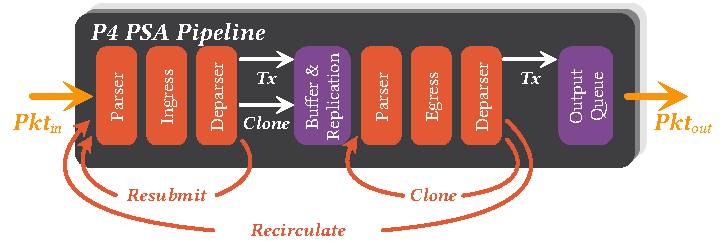
\includegraphics[width=\linewidth,keepaspectratio]{diagrams/pdp-lit/p4-psa}
	\caption[Pipeline stages and forwarding paths of the P4 PSA.]{Pipeline stages and forwarding paths of the P4 \gls{acr:psa}. User programmable blocks are coloured in orange, where \gls{acr:mat} blocks comprise the `Ingress' and `Egress' stages. While an \gls{acr:rmt}-like action model is common, the \gls{acr:psa} abstracts over how actions should be implemented in any target dataplane. Instead, it specifically determines the high-level structure of ingress and egress processing---as two separate parse-\gls{acr:mat}-deparse pipelines---and how packets may be moved and cloned between these pipelines. For instance, a packet may only be cloned at the beginning of the egress pipeline, and may only repeat processing by returning to the start of ingress. Due to this structure, some packet processing or aggregation programs may only be expressed using workarounds.\label{fig:p4-psa}}
\end{figure}

8 years on, P4 has apparently been a runaway success in much the same vein as OpenFlow, and enjoys use in production networks~\parencite{DBLP:conf/sigcomm/TianGLZCZDYMTLW21} while also enabling efficient and production-ready implementations of next-generation Internet designs such as \emph{SCION}~\parencite{DBLP:conf/conext/RuiterS21}.
These technologies, including SmartNICs, are also seeing use in national research and education networks---for control and network design such as G\'{e}ant's RARE project~\parencite{geant-rare-article}, and for fine-grained network telemetry and future P4 processing in ESnet6~\parencite{esnet6-hts,esnet6-htp}.

A more important effect of having arbitrary control over actions and manipulation of shared state is that, although limited, the set of programs we can express has grown significantly.
Although we'll discuss this in more depth in \cref{sec:offloading-and-in-network-compute}, this enables true \emph{in-network compute}---per-packet processing, e.g., in telemetry use cases like \emph{PINT}~\parencite{DBLP:conf/sigcomm/BasatRLAYM20} at rates and volumes hitherto impossible for hosts to achieve.
Moreover, this enables application acceleration and other new developments with none of the costs of host execution.

%T4P4S~\parencite{DBLP:conf/hpsr/VorosHKLTL18} converts P4 programs into C, which are linked against a target-specific network hardware abstraction layer.
%This seems to be the most effective host deployment for P4 at the moment, since it buys you DPDK-capable P4 dataplane installation compared to how terribly slow BMv2 is known to be.
%Slower than native DPDK, but outpaces OvS, and allows definition of HAL binaries in SmartNIC C code as needed too.

%?? Where does \emph{PISCES}~\parencite{DBLP:conf/sigcomm/ShahbazCPKFMR16} fit into the story? It's OvS using P4 to add new features and design dataplanes. ?? This is probably an aside.

%Ctl planes autogenerated by P4Runtime~\parencite{p4-runtime}

%Then followed up by  \gls{acr:psa}\parencite{p4-psa}.

%?? SCION~\parencite{DBLP:conf/conext/RuiterS21}

%?? Measurement like PINT~\parencite{DBLP:conf/sigcomm/BasatRLAYM20}

%?? Talk more about in-network compute?

\subsection{The return of active networking?}
The reader may well be thinking that research community has cycled back around to active networking in a new guise, and in many senses it has.
While less popular at the time, the programmable switch model we have now latched onto did in fact arise as part of this prior movement.
The remarkable observation is that if we follow the retelling of \Textcite{DBLP:journals/ccr/FeamsterRZ14}, active networking's decline was written in large part by its lack of a ``killer app''.
Of course, its main use cases at the time were touted as enabling cacheing and \gls{acr:cdn}-like behaviour, content processing, network management, and fine-grained telemetry.
These are strikingly similar to the use cases which have driven the recent upsurge of \gls{acr:pdp} applications, and in fact see real use in production edge networks~\parencite{DBLP:conf/sigcomm/TianGLZCZDYMTLW21}.
Modern measurement schemes like \gls{acr:int}~\parencite{p4-int}---covered in \cref{sec:network-monitoring}---have returned to the model of injecting per-packet actions into the packet headers themselves.

\Textcite{DBLP:journals/ccr/WetherallT19} also recognise this resurgence, and reaffirm the main drivers of \gls{acr:sdn}---\emph{economics} of a malleable software layer exploiting affordable commodity hardware (where talented software engineers are easily deployed), and \emph{virtualisation} as a tool for introducing more capability into the network.
What they don't really discuss are the concrete reasons for why the field appears to have successfully taken off this time, while it foundered before.
So, what changed?
My personal interpretation and opinion is that this arises from several angles: 
\begin{itemize}
	\item Virtualisation introduced the capability to install novel and reconfigurable packet processing to networks, but modern deployments and the constant need to `scale up' have emphasised that performance truly is a necessity. This doesn't only hark back to the logical cost involved in moving packets around the software or \gls{acr:os} stack in a machine (added latency), but also via the falloff of Moore's law~\parencite{moore-law} and Dennard scaling~\parencite{dennard-paper}. Although host capabilities have always fallen behind line-rate, they are falling even further back due to the constant, inexorable increase in Ethernet data rates.\sidenote{Of course, dedicated silicon always offers a performance edge over an arbitrary computer, at the cost of flexibility. The design, fabrication, and engineering costs are high enough that this has only ever really been justified in common use-cases (e.g., firewalls and \glspl{acr:ids}) or where there really is a business case as with modern hypergiant providers.} `Line-rate' has increased from its initial \qty{10}{\mega\bit\per\second} to \qty{1}{\giga\bit\per\second}~\parencite{gbe-standard}, to \qty{100}{\giga\bit\per\second}~\parencite{100-gbe}, with ongoing work to standardise \qty{400}{\giga\bit\per\second} links. When we consider that Ethernet frame sizes have in the same period expanded on \emph{some} deployments from \qty{1560}{\byte} to \qty{9000}{\byte} `jumbo' frames, it is plainly visible that per-packet processing deadlines simply cannot be met by commodity hosts on smaller packets.
	
	\item The unforeseen capabilities, reach and business needs of hypergiant network operators such as Google and Meta, pushing the boundaries of scalability~\parencite{DBLP:conf/sigcomm/GigisCMNKDKS21}, have also played a key role. Crucially, their business needs include not only the administration of such large networks but also rely on accelerating cloud compute workloads, large-scale \gls{acr:ml} model training and inference, and distributed computation within their datacentre networks. As we'll cover in \cref{sec:offloading-and-in-network-compute}, in-network compute allows specific optimisations for these tasks: for instance gradient aggregation in-network, or \glspl{acr:cca} managed co-operatively by the routing infrastructure. In single-owner environments such as these, all aspects of distributed computation can be controlled and optimised, so such hyper-converged infrastructure is not only possible but necessary from an economic standpoint---particularly when in-network compute becomes the only available road to greater performance. While such companies have the capability and precedent to develop their own hardware---e.g., network-connected accelerators like Microsoft \emph{BrainWave}~\parencite{DBLP:conf/isca/FowersOPMLLAHAG18}---these organisations already had an abundance of engineers familiar with \gls{acr:sdn} who were poised to make great use of the joint flexibility and performance offered by \glspl{acr:pdp}.
\end{itemize}
Alternatively, we might argue that it is the control plane innovations of \gls{acr:sdn} that made this possible in the first place; beforehand, the design schism of capsules versus programmable switches was indeed an open question (one might say between `pragmatic' and `interesting' approaches to the task).
The field's re-evolution of programmable switches (and now \glspl{acr:nic}) offers a healthy does of pragmatism, ensuring that today's model is performant---but it is almost entirely focussed on allowing runtime reconfigurable specificity over which packets are fed to a pre-set menu of dataplane programs, as opposed to totally arbitrary packet-level programs.

%?? Fit into above some mention of `obvious throwbacks' like \emph{TPP}~\parencite{DBLP:conf/sigcomm/JeyakumarAGKM14}

%?? Fit this in wrt. moore's law observations.
%?? How? They believed the way to make it feasible was to limit scope to management. Now we knoe this is valid, but so too is in-network compute?
Yet the model of in-network compute we have converged on remains radically different from early estimates, even though it may feel like the community is simply retreading the concept of `programmable switches'.
Consider the motivation behind \emph{SmartPackets}:
\begin{quotation}
	\noindent
	%	A major motivation behind Active Networks was the theory that there is an exponential growth of computing power in the network suggested by Moore’s Law, which states that the speed of electronic components doubles every 18 months.
	%	Unfortunately, in most parts of the Internet, the traffic growth rates far exceed the growth rate of Moore’s Law. ...
	%	There are places, however, where Moore’s Law is winning.
	%	One place is network management and monitoring.
	%	The average device is not generating, processing, or receiving drastically more network management traffic than it was a year or two ago.
	%	We can hope, therefore, that there is more per-device processing power available for network management than there was in the past.
	%	A major motivation behind Active Networks was the theory that there is an exponential growth of computing power in the network suggested by Moore’s Law, which states that the speed of electronic components doubles every 18 months.
%	Unfortunately, in most parts of the Internet, the traffic growth rates far exceed the growth rate of Moore’s Law. ...
	There are places, however, where Moore’s Law is winning.
	One place is network management and monitoring.
	The average device is not generating, processing, or receiving drastically more network management traffic than it was a year or two ago.
	We can hope, therefore, that there is more per-device processing power available for network management than there was in the past.
	
	\strut\hfill\parencite[p. 68]{DBLP:journals/tocs/SchwartzJSZRP00}
\end{quotation}
At that time too, Moore's law was insufficient to allow per-packet processing at cutting-edge Ethernet speeds (before its falloff really came to pass).
As such, the only time that \emph{full, general-purpose compute} could be deployed in this context was when the infrastructure had already aggregated or reduced the data frequency in some way.
The authors here make two key, and arguably fatal, assumptions.
The first hinges on a perceived status quo: that management and telemetry data would \emph{and must} remain low-frequency (e.g., flow-level, link-level, or sampled measurements).
\Cref{sec:offloading-and-in-network-compute} shows that for many applications this cannot be the case, as per-packet processing and telemetry are essential in accelerating distinct use cases and diagnosing insidious network faults and behaviours such as microbursts.
The second is that the compute model itself should be equivalent to host machines, able to express any packet processing programs an engineer might dream of.
We see this in other programmable switch proposals of the era~\parencite{DBLP:journals/jsac/WolfT01}, but time has shown that \gls{acr:npu}-like SmartNICs of today can only achieve this for one or two ports---let alone the full fanout of a rack-mounted switch.
The first key difference lies in how, at scale, we must make use of advanced (though highly programmable) \glspl{acr:asic} rather than full-fledged \glspl{acr:cpu}.
While the design of SmartNICs allows us to dispel the first assumption and enables exciting new use cases, in the switch form factor we have come to accept \emph{constrained}, yet still capable, programmability to meet line-rate processing.
The other key difference between the modern \gls{acr:pdp} ecosystem and active networks is that the scope of deployment has narrowed considerably.
While early proponents dreamed of a fully participative network, inclusive of end-hosts' in-network programs, \gls{acr:pdp} devices must be programmed ahead-of-time and managed by an attached controller machine---both for performance and for management of the associated control-plane machinery such as \gls{acr:mat} structure.
In turn, deployment of in-network compute has become far more insular, and effectively bound to the \gls{acr:as} level.
%?? Bound to the \gls{acr:as} level. Insular.

%?? What's different? Focus on ctl-plane connected, but essentially limited to individual \glspl{acr:as} in contrast to the augmented end-to-end vision of yore. Did it succeed \emph{because} it's more constrained? i.e. no inter-AS vision, not tied to preselected forwarding paths...
%
%?? Regardless, the old paradigm of active networking has been realised in the form of \glspl{acr:pdp} and in-network compute.

\subsection{Frontiers in programmable networks}\label{sec:frontiers-in-programmable-networks}
Commercial developments along the same lines as this modern \gls{acr:pdp} hardware are proceeding apace as network bandwidth demands grow larger.
Intel's Tofino 2~\parencite{tofino2} represents the latest product in the lineage of \gls{acr:rmt} hardware, offering \qty{12.8}{\tera\bit\per\second} with support for \qty{400}{\giga\bit\per\second} Ethernet.
Nokia's FP5~\parencite{nokia-fp5} similarly promises full programmability for high-density switching and routing at \qty{800}{\giga\bit\per\second} Ethernet, while Intel's \emph{infrastructure processing units}~\parencite{intel-ipu} present a combined \gls{acr:fpga}- and Xeon-based series of SmartNICs for accelerating datacentre applications.
However, there is still concerted research effort in further developing the tooling used to program these devices and in how future hardware designs might evolve to incorporate new models of packet processing.

%?? Mention more recent lang and HW developments.
%?? Tofino 2~\parencite{tofino2}---\qty{12.8}{\tera\bit\per\second} with support for \qty{400}{\giga\bit\per\second} Ethernet.
%?? Nokia's fabric?~\parencite{nokia-fp5}
%?? Intel's other new thing Dimitris mentioned?~\parencite{intel-ipu}

\paragraph{Language design}
At present, P4 and the \gls{acr:psa} are restrictive in the sense that the only events which can drive user-provided code are packet arrivals and departures.
Event-driven languages have been suggested~\parencite{DBLP:conf/hotnets/IbanezABM19}, built on the need for timer, link state, and queue state events to enable useful applications.
Workarounds in P4 exist to emulate these capabilities, such as queue size estimation and costly packet recirculations, but these inflate the amount of state needed by applications or incur their own runtime penalities.
The authors explicitly incorporate these events into the pipeline model and modify the P4 language to support their processing by additional logical pipelines; however, this demands hardware support in non-NetFPGA environments.
%Timer events and device state changes would empower in-network RL use-cases, signalling timesteps for RL agents or new, effective, fine-grained sources of input state.
\emph{Lucid}~\parencite{DBLP:conf/sigcomm/SonchackLRW21} builds a new, high-level language which expresses many of these capabilities by compiling down to the P4-\gls{acr:psa} architecture.
In particular, it allows for event handlers to be triggered between devices while enabling more flexible control and modification of shared datastructures behind reliability measures like fast reroute.

The P4 language is currently incompatible with heterogeneous hardware to some extent; written dataplane programs are typically tied to a particular switch model, for instance V1Model, \gls{acr:psa}, NetFPGA SUME, or the Tofino Native Architecture.
Network architects typically procure hardware from several manufacturers to prevent vendor lock-in, but the P4 model for each device has its own metadata types, hardware constraints, and quirks which developers must be aware of.
While architectures such as the \gls{acr:psa} are more general and should, in principle, support several target switches, it is often preferable to use a switch's own architecture for performance or optimisation reasons.
As a result it is currently tedious to write and maintain a unified dataplane that is provably uniform across different packet processing devices.
$\mu$\emph{P4}~\parencite{DBLP:conf/sigcomm/SoniR0DF20} extends the P4 compiler to decompose parser and action code into independent subprograms which may be composed together in a more simple manner by programmers.
This simplifies porting behaviours between different switch models---particularly in separating out (and integrating) complex interactions and dependencies between parser, deparser and action code stages.
\emph{Lyra}~\parencite{DBLP:conf/sigcomm/GaoZLMZTSCZY20} is a language for running switch programs e.g., P4 and Broadcom's \emph{NPL}~\parencite{broadcom-npl}, across heterogeneous switch hardware, while also handling placement constraints.
Lyra expresses the entire network dataplane using the `one big switch' abstraction, and compiles from its own higher-level language to an \gls{acr:ir} and then to P4 or NPL.
Compilation is combined with topology information about the target network, as well as placement constraints, to generate an optimal embedding in the network using a \gls{acr:smt} solver.

As is the case when programming host machines, verifying that a dataplane program behaves correctly---both within a single switch and the wider dataplane with regards to code and \gls{acr:mat} contents---presents its own set of challenges.
In particular, fully programmable dataplanes enable new classes of bugs such as header malformations which existing network verification tools are not designed to handle.
This is complicated further still by the fact that a P4 program's operation is determined also by the control plane and the contents of its \glspl{acr:mat}.
\emph{P4-NoD}~\parencite{mckeown2016automatically} is an earlier solution to the problem, translating invariants into Datalog for verification by older tooling while modelling correctly emitted packets via pairwise `packet acceptance' constraints between switches.
\emph{p4v}~\parencite{DBLP:conf/sigcomm/LiuHSSLSWCMF18} combines guarantees about the bounds of control plane values with expected output invariants to detect counter-example packets using an \gls{acr:smt} solver.
\emph{bf4}~\parencite{DBLP:conf/sigcomm/DumitrescuSNR20} endeavours to make the annotation task considerably easier for programmers, again relying on \gls{acr:smt} solvers to also produce control plane rule filters and candidate bug fixes.
\emph{Aquila}~\parencite{DBLP:conf/sigcomm/TianGLZCZDYMTLW21} achieves a similar class of \gls{acr:smt}-solver based verification, using a new language which makes it easier to express dataplane invariants across one or more switches.
Aquila further innovates by using \gls{acr:smt} counterexamples to localise likely locations and fixes for bugs, as well as developing numerous domain-specific optimisations to generated logical formulae.

\paragraph{Hardware design}
While the pipelined model of the \gls{acr:psa} is undeniably effective, it can be restrictive for many classes of dataplane program; for instance cases where processing is based on more than raw packet events, or where more complex dataflow is required between functions.
\emph{PANIC}~\parencite{DBLP:conf/hotnets/StephensAS18} offers one solution by placing a routing fabric between distinct packet and data processing elements in a SmartNIC.
These compute elements (mixed \glspl{acr:rmt}, \gls{acr:fpga} blocks and accelerators) are connected in a tiled architecture, each containing a router to direct packets to their intended internal destination.
Such a design would enable general, asynchronous, and novel compute in SmartNICs and switches, for instance offering consistent and easy to use communication between workers versus hard-coded \gls{acr:me} relationships or ordering dependencies between subprograms across pipelines.

In multitenant environments such as data centres or cloud compute providers, clients may wish to take advantage of \gls{acr:pdp} hardware if it is present---between pairs of virtual servers, for instance.
Recalling the single pipeline design of the \gls{acr:psa}, it's clear that this is a difficult resource sharing problem between \glspl{acr:mat}, pipeline width and stages, and per-packet metadata storage.
Moreover, ensuring that applications cannot interfere with one another's performance guarantees, state, or the forwarding behaviour of all packets is non-trivial (i.e., a malicious table might force infinite packet recirculation)---particularly when tables or logic might be reused between user pipelines to save such resources.
%?? difficult resource sharing problem ?? the \gls{acr:psa} 
Alternative architectures have been presented to make this task simpler.
The above \emph{PANIC} has been revised and recast as a solution to this multitenancy problem~\parencite{DBLP:conf/osdi/LinPSSA20}, losing much of the flexibility of its initial iteration to accelerate this use case.
(Multitenant) PANIC now uses a single ingress \gls{acr:rmt} pipeline to tag packets with all hops of their intended offload chain, while compute units (\glspl{acr:asic} and RISC-V \glspl{acr:cpu}) pass packets between one another using an all-to-all direct crossbar.
Higher-level rate limits are controlled by a programmable \gls{acr:pifo} scheduler~\parencite{DBLP:conf/sigcomm/SivaramanSACCAB16} to enforce \gls{acr:qos} around shared offload blocks.
However, relying on only the ingress \gls{acr:rmt} to determine such routes leads to potentially inflexible packet processing chains.
\emph{MTPSA}~\parencite{DBLP:conf/conext/StoyanovZ20} instead extends the \gls{acr:psa} to place client code into a set of inner `user' pipelines between the egress parser and \glspl{acr:mat}.
Each runs its own code, and applies Unix's read-write-execute privilege model to resources, fields, tables and \texttt{extern}s to limit per-program access capabilities.
The standard ingress and egress pipelines are designated as `super-users', who determine the user pipeline to execute and are responsible for higher-level forwarding.
This approach is rather coarse-grained, and prohibits reuse of tables (increasing per-user resource costs).
In addition, restricting pipeline placement to egress-only limits program expressibility---operations such as changing the output port are illegal for user code.

While P4 registers enable useful stateful programming, concurrent access semantics and pipeline ordering restrictions can make some applications difficult to express.
Equally, their implementation in any platform relies on platform-specific \texttt{extern}s according to the \gls{acr:psa}, and as such their semantics and correct operation will vary on a target by target basis.
Architectures such as \emph{Banzai}~\parencite{DBLP:conf/sigcomm/SivaramanCBKABV16} and its accompanying C-like language \emph{Domino} compile to \glspl{acr:mat} internally from restricted \emph{packet transactions}.
They differ from \gls{acr:rmt} by having each action unit (or \emph{atom}) additionally contain a memory unit for shared state, which only it may access (rather than the global, shared registers of P4).
Atoms contain a variety of \gls{acr:alu} blocks to enable 1-cycle updates and reads on branches as required for safe concurrent state processing.
Domino's restrictions are close to those of \gls{acr:ebpf} programs, with the extra limitation that only one entry may be accessed per array; the compiler is responsible for building and allocating \glspl{acr:mat} and concurrently sequencing all transactions.
This explicit focus on \numrange{1}{2} cycle logic blocks allows Banzai to guarantee line-rate execution.
\emph{FlowBlaze}~\parencite{DBLP:conf/nsdi/PontarelliBBCSB19} targets instead \emph{per-flow} state for L2--L4 traffic, mixing \gls{acr:mat} blocks with custom extended \gls{acr:fsm} units.
These extended \glspl{acr:fsm} store variables, can read and modify global registers, and use \glspl{acr:mat} to look up simple state transition functions based on fields of all accessible state.
States are stored on a per-flow basis, allocated from a hardware-backed hash table.
While \glspl{acr:mat} and \gls{acr:fsm} blocks may be interposed freely to express more varied programs, true flexibility is only possible at present when these blocks may be easily replaced (i.e., in an \gls{acr:fpga} environment).
This flexibility has a sharp downside; the variable and state model forces pipeline stalls to clear up hazards around concurrent \gls{acr:fsm} state accesses, leading to packet drops and sub-line-rate packet processing for some dataplane functions.

%?? Sim between these and RMT? atoms -- instrs exec in 1--2 cycles.

%?? Taurus moved out of representations section~\parencite{DBLP:journals/corr/abs-2002-08987,DBLP:conf/asplos/SwamyR0GO22}
Although \gls{acr:ml} can be made feasible in \gls{acr:pdp} hardware as I show in \cref{sec:inc-uses-pdp-ml}, achieving more complex or higher-precision inference at line rate can only be enabled by dedicated architectural support.
\emph{Taurus}~\parencite{DBLP:journals/corr/abs-2002-08987,DBLP:conf/asplos/SwamyR0GO22} is a proposal to add compute and memory units to the \gls{acr:psa} as part of a map-reduce block specifically designed to optimise per-packet \gls{acr:ml} inference.
The proposal has the ingress \gls{acr:rmt} pipeline now perform feature extraction from packet header data among its standard duties.
In particular, it demonstrates that efficient line-rate inference can work using a \gls{acr:cgra} of map-reduce units between the ingress and egress pipelines---implementing \glspl{acr:nn}, \gls{acr:lstm} networks, or \glspl{acr:svm} which process every packet header vector.
This \gls{acr:cgra} implements a large grid of replicated fixed-point compute and memory units, allowing higher throughput by what the authors describe as `spatial \gls{acr:simd}'.
This achieves line-rate throughput while reducing latencies from the $\mathcal{O}\left(\unit{\milli\second}\right)$ \gls{acr:cpu} and \gls{acr:gpu} inference to $\mathcal{O}$(\qty{e2}{\nano\second}), dependent on the target application.
In turn, the outputs of any classifiers in this block become available to later pipeline stages, which are able to act upon packets accordingly.
Training \gls{acr:ml} models online using Taurus requires that input packets are sampled alongside local signals such as per-flow \gls{acr:qos} metrics to be directed towards a cooperating host machine in the control plane, and cannot be performed unassisted (i.e., purely on-device).

Access to the host programming stack and its full feature set remains an attractive prospect, even subject to the costs discussed throughout \cref{sec:offloading-and-in-network-compute}.
\gls{acr:nic}-\gls{acr:cpu} co-designs present a more exotic solution to the latter problem, deeply integrating these two elements together in stark contrast to the typical `peripheral' view of the \gls{acr:nic}.
Primarily motivated by optimising around the growing prevalence of \unit{\micro\second}-level \glspl{acr:rpc} in data centres, \emph{\textsc{NeBuLa}}~\parencite{DBLP:conf/isca/SutherlandGFMPD20} eliminates the \gls{acr:pcie} interconnect between the \gls{acr:nic} and \gls{acr:cpu}, placing received packets directly into the L1 cache of a target \gls{acr:cpu} core.
This relies mainly upon exclusively using a connectionless \gls{acr:rpc} transport which enforces fail-fast behaviour for requests which will miss their deadline, allowing shared buffers for \emph{all connections} to be shrunk to fit into L3 cache.
The integration of \gls{acr:nic}-to-core steering with the L3 cache then allows correct routing to the relevant L1 cache slot for the target \gls{acr:cpu} core.
Base packet forwarding times are thus reduced below \qty{100}{\nano\second}.
%?? load-balancing between such cores in L3 cache, which holds whole buffer ?? shrunk buffers due to connectionless \gls{acr:rpc} transport -> shared queues, early fail delay-sensitive \glspl{acr:rpc} if too loaded. ?? integ of nic-to-core steering and cpu allows L1!
\emph{nanoPU}~\parencite{DBLP:conf/osdi/IbanezMAJ0KM21} takes this concept further to serve packets directly into the register file of a target core using a thread-safe interface, reducing packet handover times to a minimal \qty{69}{\nano\second} \gls{acr:rtt} (\qty{17}{\nano\second} excluding \gls{acr:mac}).
To enable this, custom transport protocol logic is implemented in hardware, and packets are classified and further modified at line rate with the aid of \gls{acr:psa} ingress and egress pipelines.

%?? Are the tools just sharper now?

While the P4 \gls{acr:psa} is a compilation target supported on many SmartNICs, in many ways it is a suboptimal model as it ignores the constraints and strengths of \gls{acr:nic} hardware compared to \gls{acr:rmt} switches.
The \emph{Portable \gls{acr:nic} Architecture}~\parencite{p4-pna}, which is in the process of being codified, offers first-class support for such devices, using instead a single pipeline aided by \texttt{extern}s for host$\leftrightarrow$\gls{acr:nic} processing.
This is expected to feature a message processing block for programmable segmentation and coalescing etc., as expected by host \glspl{acr:os} and their drivers.
Most notably, this includes device-local updates and additions to table state, packet mirroring, and table row expiry events.
To date, device-local updates have been implemented as part of T4P4S to explore some of the design-space around concurrent table access and modifications~\parencite{DBLP:conf/ancs/SimonSSGC21}.
However, this capability is not guaranteed for all similar devices.
Netronome \gls{acr:nfp} \gls{acr:nic} tables are reliant on the optimised DCFL~\parencite{DBLP:conf/infocom/TaylorT05} data format, potentially still limiting the capability for rule installation to control plane devices.

%\gls{acr:pdp} hardware excels in applying actions to network packets using \glspl{acr:mat}, potentially giving us a high-performance method to install selected actions within the network.
%However, directly modifying these match tables from within the device itself is neither feasible nor safe.
%On Netronome \gls{acr:nfp} hardware in particular, rule updates \emph{must} be applied by the co-hosted controller machine, as tables are reliant on the optimised DCFL~\parencite{DBLP:conf/infocom/TaylorT05} data format.
%In addition to the prohibitive complexity of building this data structure on-device, its construction requires knowledge of the entire rule set (and cannot be incrementally updated).

\section{Offloading and in-network compute}\label{sec:offloading-and-in-network-compute}
%?? Explain rationale first...
As we've explored in \cref{sec:from-fixed-function-to-fully-programmable,sec:modern-pdps}, modern networks now have a large variety of tools to enable traffic and packet processing, including hosts, programmable switches, SmartNIC devices, and middleboxes---all in tandem with control plane programmability.
%?? Diverse set of devices having different perf characteristics in latency/tput, reachability, prioce points, degrees of programmabiklity
This diverse set of devices also means that market silicon now offers a wide variety in performance characteristics such as latency and throughput, connectivity, price points, and degrees of programmability.
%Explain \cref{fig:pdp-lit-steering} more fully in-text
%?? (a) has some benefits: if both close to each other, then most of path is the same---key for CDNs, DDoS scubbing etc. or when we want to use PDP provided by others' infra.
%?? (b) is a necessity -- pkts must be moved away 
%?? (c) can be bump-in-wire host or dedicated device, but minimum impact on path. Or AS. When can (c) not be achieved?
Accordingly, network architects must also consider how best to integrate \glspl{acr:nf} backed by these capabilities into their networks.
Consider \cref{fig:pdp-lit-steering}: to minimise extra latency costs imposed on carried traffic as well as control plane complexity, we want to minimise the amount of \emph{traffic steering} required.
In the worst case, traffic may need to be routed to another organisation to make use of high-volume services like \gls{acr:ddos} traffic scrubbing, \glspl{acr:cdn}, or \gls{acr:pdp} capabilities exposed by cloud compute\sidenote{These classes of service tend to have enough geographical replication that the network function and the target server are reasonably close to one another, for instance in proximity to a shared \gls{acr:ixp}. As such, users' paths to both nodes are likely to be similar, the last few hops excepted.} (\cref{fig:pdp-lit-steering:off}).
Steering within \glspl{acr:as} as in \cref{fig:pdp-lit-steering:semi-on} is a necessity to enable \gls{acr:vnf} chaining between host machines in a way which is reliably reconfigurable, but this naturally increases routing and processing latency as well as bandwidth demands in the \gls{acr:as} in question.
The only way to eliminate steering costs completely is to place dataplane programs \emph{on-path} (\cref{fig:pdp-lit-steering:on})---but this has key drawbacks.
If we place commodity hosts in-line like this, then they will be unable to meet line-rate demands in faster networks; we have also given up the flexible reconfiguration and horizontal scalability that steering bought us.
\gls{acr:pdp} innovations like programmable \gls{acr:asic}-backed switches and SmartNICs are the best tools for performing processing here, but not every application can be run in these locations due to the limits of their respective compute models.

\begin{figure}
	\centering
	%	\resizebox{\linewidth}{!}{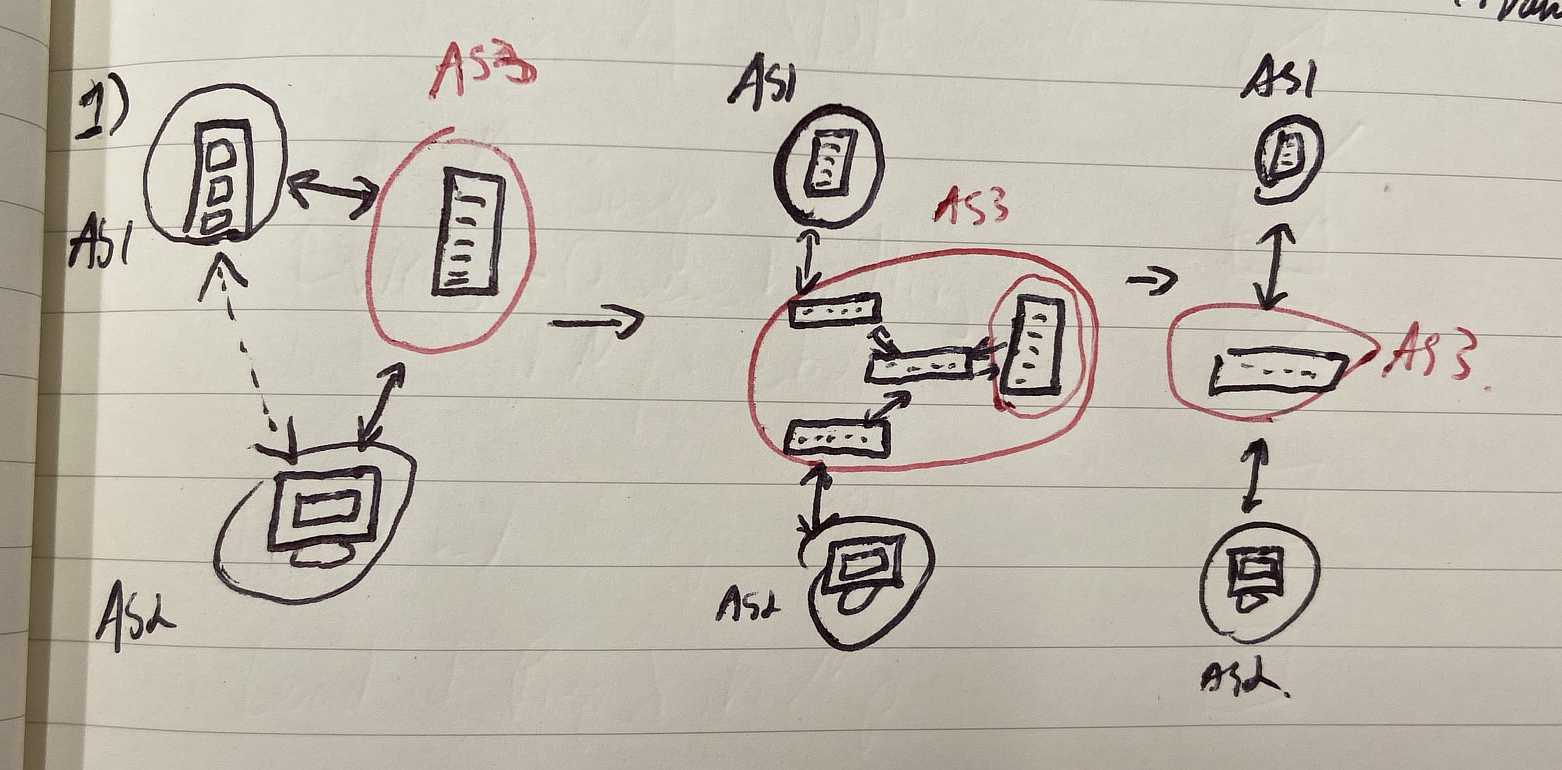
\includegraphics{diagrams/pdp-lit/steering-draft}}
	\begin{subfigure}{0.49\linewidth}
		\resizebox{\linewidth}{!}{\begin{tikzpicture}
	\node[draw, circle, color=uofgslate, label=left:{\gls{acr:as} 1}] (server) {
\includegraphics[width=1cm, height=1cm, keepaspectratio]{diagrams/cisco-icons/standard host}};
	\node[draw, circle, color=uofgslate, label=left:{\gls{acr:as} 2}] at ($(server) + (0,-4)$) (client) {
\includegraphics[width=1cm, height=1cm, keepaspectratio]{diagrams/cisco-icons/pc}};
	\node[draw, circle, color=uofgslate, label=right:{\gls{acr:as} 3}] at ($(server) + (2,-1)$) (scrub) {
\includegraphics[width=1cm, height=1cm, keepaspectratio]{diagrams/cisco-icons/ios firewall rust}};

	\draw[<->, thick, color=uofgslate, dashed, out=260,in=90] (server) to node[left] {Shortest path} (client);
	\draw[<->, thick, color=uofgrust, out=90,in=200] (client) to node[right] {Taken path} (scrub);
	\draw[<->, thick, color=uofgrust] (server) to (scrub);
\end{tikzpicture}}
		\caption{Off-path.\label{fig:pdp-lit-steering:off}}
	\end{subfigure}
	\begin{subfigure}{0.49\linewidth}
		\resizebox{\linewidth}{!}{\begin{tikzpicture}
	\node[draw, circle, color=uofgslate, label=left:{\gls{acr:as} 1}] (server) {
\includegraphics[width=1cm, height=1cm, keepaspectratio]{diagrams/cisco-icons/standard host}};
	\node[draw, circle, color=uofgslate, label=left:{\gls{acr:as} 2}] at ($(server) + (0,-6)$) (client) {
\includegraphics[width=1cm, height=1cm, keepaspectratio]{diagrams/cisco-icons/pc}};

	\node at ($(server) + (1,-2)$) (sw1) {
\includegraphics[width=1cm, height=1cm, keepaspectratio]{diagrams/cisco-icons/router}};
	\node at ($(server) + (1,-4)$) (sw2) {
\includegraphics[width=1cm, height=1cm, keepaspectratio]{diagrams/cisco-icons/router}};
	\node at ($(server) + (2.5,-3)$) (sw3) {
\includegraphics[width=1cm, height=1cm, keepaspectratio]{diagrams/cisco-icons/router}};

	\node at ($(sw3) + (2,0)$) (scrub) {
\includegraphics[width=1cm, height=1cm, keepaspectratio]{diagrams/cisco-icons/ios firewall rust}};

	\begin{scope}[on background layer]
		\draw[color=uofgslate] (sw3) ellipse (3cm and 1cm);
	\end{scope}
	\node at ($(scrub) + (0, 1.25)$) {\gls{acr:as} 3};

	\draw[<->, thick, color=uofgrust, out=90,in=240] (client) to (sw2);
	\draw[<->, thick, color=uofgrust, out=60,in=240] (sw2) to (sw3);
	\draw[<->, thick, color=uofgrust, out=120,in=300] (sw3) to (sw1);
	\draw[<->, thick, color=uofgrust, out=120,in=270] (sw1) to (server);

	\draw[<->, thick, color=uofgrust, out=30,in=150] (sw3) to (scrub);
	\draw[<->, thick, color=uofgrust, out=330,in=210] (sw3) to (scrub);

	\draw[<->, thick, color=uofgslate, dashed] (client) to (sw2);
	\draw[<->, thick, color=uofgslate, dashed, shorten >=-0.12cm,shorten <=-0.12cm] (sw2) to (sw3);
	\draw[<->, thick, color=uofgslate, dashed, shorten >=-0.12cm,shorten <=-0.12cm] (sw3) to (sw1);
	\draw[<->, thick, color=uofgslate, dashed] (sw1) to (server);
\end{tikzpicture}}
		\caption{On-\gls{acr:as}-path (steering).\label{fig:pdp-lit-steering:semi-on}}
	\end{subfigure}
	
	\begin{subfigure}{0.65\linewidth}
		\resizebox{\linewidth}{!}{\begin{tikzpicture}
	\node (server) {
\includegraphics[width=1cm, height=1cm, keepaspectratio]{diagrams/cisco-icons/standard host}};
	\node at ($(server) + (2,0)$) (scrub) {
\includegraphics[width=1cm, height=1cm, keepaspectratio]{diagrams/cisco-icons/programmable switch rust}};
	\node at ($(scrub) + (2,0)$) (client) {
\includegraphics[width=1cm, height=1cm, keepaspectratio]{diagrams/cisco-icons/pc}};

	\draw[<->, thick, color=uofgrust, out=30,in=150] (server) to (scrub);
	\draw[<->, thick, color=uofgrust, out=30,in=150] (scrub) to (client);

	\draw[<->, thick, dashed, color=uofgslate, out=330,in=210] (server) to (scrub);
	\draw[<->, thick, dashed, color=uofgslate, out=330,in=210] (scrub) to (client);
\end{tikzpicture}}
		\caption{On-path (direct).\label{fig:pdp-lit-steering:on}}
	\end{subfigure}
	\caption[The spectrum of on-path traffic processing.]{To introduce packet processing to the network, engineers must make a conscious decision about where such processing may be installed, and if needed how traffic can be steered there---this leads to spectrum of how on-path processing may be. The main sizes and types of redirections are shown here: (a) having to redirect to another network for packet processing, (b) internally rerouting and steering packets to reach one or more processing machines (e.g., in \gls{acr:vnf} scenarios), and (c) placing processing \emph{directly in-path}. Generally speaking, smaller path deviations have a smaller latency impact. Paths and \gls{acr:as} relationships here are purely for demonstration, and may be longer in practice (similarly, case (b) may occur entirely within a single data centre \gls{acr:as}). Appliances performing packet processing are coloured {\color{uofgrust} in orange-red}.\label{fig:pdp-lit-steering}}
\end{figure}

These new, specialised devices are a double-edged sword---making efficient use of \emph{all} network resources becomes non-trivial due to device heterogeneity in architecture and capabilities.
Ideally, we want to maximise the number of packets which are served by on-path, in-network functions such as in \cref{fig:pdp-lit-steering:on}.
Even when using consistent programming models like P4, using all of a device's capabilities is difficult, requiring hardware-specific expertise, experience, and microarchitectural knowledge.
At the same time, organisations would prefer to accelerate the code they already have rather than re-architect solutions from the ground up.
%Operators and engineers can choose from these according to their needs, enabling new in-network use cases, but this is also something of a double-edged sword.
%?? Double-edged sword: how to use it all?
Can we then accelerate \emph{individual parts} of a packet processing stack?

%?? Such power is a double edged sword; how to use. Difficult; expertise, training, microarchitectural knowledge and experience, languages...
%?? Not just all of a packet program, but at the granularity of *parts* of such a program
%?? Notion extends within the host stack, also
%?? Offloading was originally used to refer to simple accelerations which could be delegated to the hardware to free up host machine resources: packet splitting to MTU size, diving requests among coresa (RSS), and checksumming at various levels
%?? Maximise proportion of traffic served by best-case deplyoments

%Offloading: Moving part or all of a program to execute elsewhere (why? improved latency, perf, tput, take advantage of existing heterogeneous hardware). Good even if just partial: especially if slow path is uncommon. I.e., early-exit good. Can be in-host, or between host and devices. OR to fall back to a more capable/accurate computation env. Relate to above: enables routing through low-latency, high-tput in-network routes.

\emph{Offloading} is the process of moving part or all of a packet processing function elsewhere to improve overall performance---reducing latency or increasing throughput---typically by taking advantage of novel heterogeneous hardware.
Originally, this referred to simpler transport-level accelerations that \glspl{acr:nic} could perform in hardware which would free up \gls{acr:cpu} cycles on a host machine, such as checksum offloads, large send \& receive offloads to split or coalesce larger than \gls{acr:mtu}-size packets, and receive-side scaling.
The idea is that the unique capabilities of existing \gls{acr:sdn} switches and \gls{acr:pdp} hardware can be taken advantage of to optimise a target dataplane, enabling a very generic and useful kind of acceleration.
This extends also to host machines, which have no shortage of technologies for improving packet processing by shifting user code into the network stack or skipping the kernel entirely.
Such hosts may even use attached SmartNICs to accelerate applications or transport logic.

For argument's sake suppose that we want to process packets using a firewall, followed by a primitive statistical or \gls{acr:ml} model, and followed again by a \gls{acr:dpi} block whenever the second stage emits a warning.
Naturally, the simplest deployment is to have all three functions installed on host machines, but this is also the most wasteful.
While I'll introduce specific examples later, the only function here which would currently require a host machine would be the final \gls{acr:dpi} block; even then, this is only required by a small subset of packets which trip an earlier-stage alarm.
As such, routing all packets through a \gls{acr:vnf} chain imposes steering and the higher latency costs of host-based execution upon all packets, to say nothing of the reduced throughput per box.
A more optimal solution is to install the firewall rules into the \gls{acr:tcam}-backed \glspl{acr:mat} of commodity switches, which \emph{can} perform these checks at line-rate, and to offload the statistical logic into similarly on-path programmable switches or \glspl{acr:nic} at a lower arithmetic precision.
In this case we have a hardware-accelerated fast path without any unneeded steering, while only packets which need to fall back to a more capable or accurate computation environment take the (less likely) slow path.

%The concept of offloading extends also to host machines, where...
The key problem is that automatically offloading arbitrary functions is an open research challenge.
Different devices expose different programming models and languages, and have unique capabilities and limitations; additional or missing \glspl{acr:fu}, code store size limits, bespoke threading models, and other resources.
\gls{acr:pdp} devices have additional constraints on reconfiguration: firmware installation can take from seconds to minutes, limiting a chain's pliability as nodes cease to function for extended periods of time without ample provisioning to handle transition states.
Individual functions are also tricky to interconnect (i.e., passing variable state between \gls{acr:nf} stages), to compute the ideal layout of in the network, and to provision in even single tenant scenarios.
%?? tricky to interconnect, layout, provision.

\emph{In-network compute} is a concept connected to offloading, exploring novel applications which can be enabled or made scalable entirely through \gls{acr:pdp} hardware.
Rather than moving subprograms and arbitrary logical snippets down the stack, in-network compute seeks to move dedicated, complex, or involved applications onto \gls{acr:pdp} hardware, asking how to take advantage of intrinsic capabilities of dataplane devices.
Such research demands more careful exploration in algorithms and data formats, pushing the limits of what programs may be expressed in restricted environments such as P4.
What makes this an exciting area of study is that in-network applications are often defined by a tangled net of benefits and costs.
Suppose in \cref{fig:pdp-lit-steering:on} the two endpoint machines first check or update state using another service (e.g., a key-value store) before communicating with one another.
By moving this service \emph{completely into the \gls{acr:pdp} infrastructure}, entire \glspl{acr:rtt} worth of communication delay can be eliminated.
In data centre networks, where \glspl{acr:rtt} are already $\mathcal{O}\left(\unit{\micro\second}\right)$, simply placing a host in-line would undo most of this latency reduction\sidenote{While host offloading frameworks have come a long way, there are data transfer costs which cannot be elided which we'll discuss in the sequel.} while being unable to meet rack-scale fanout.
This becomes key when dealing with \gls{acr:rpc} workloads common to such data centres, where completions and \glspl{acr:rtt} are on an $\mathcal{O}\left(\unit{\micro\second}\right)$ timescale themselves~\parencite{DBLP:journals/cacm/BarrosoMPR17,DBLP:conf/nsdi/KaliaKA19,DBLP:conf/isca/SutherlandGFMPD20}.
Further example services may also aggregate data from many sources to allow a single host to process it, or apply per-packet \gls{acr:ml} inference at line rate; when end-hosts and the network fabric are all jointly owned, there is great scope for tighter network-application integration and what it might enable.
Notably, handcrafted in-network services such as \gls{acr:ml} inference might replace entire blocks in an \gls{acr:nf} chain, better supporting \gls{acr:vnf} offloading by making clever use of the underlying hardware.
The costs incurred by such services are also interesting.
In-network \gls{acr:ml} must sacrifice accuracy---the lack of \glspl{acr:fpu} in network hardware forces implementers to employ fixed-point arithmetic or other data formats.
Not all programs may be moved down to \gls{acr:pdp} hardware unaltered.

%-- eliminate entire services (eliminating one or more RTTs), data aggregation to enable the work of host machines, or... ?? typifcally when both ends owned by same operator? ?? tighter integration w/ appliocations, or what is enabled by it.

%?? elim RTTs -- DC scale on order micros with RPC-type workloads -- every us counts so can't e.g. host.

%?? INC includes capabilities which enable offload. i.e., accel'd ml
%
%?? focus on what can be enabled that takes adv. of specific, intrinsics of dataplane devices
%?? less on arbitrary compute
%?? studies the tradeoffs needed to install in these envs
%?? installation of entire services
%?? pushing the limits of what can be expressed in restricted envs like P4 -- handcrafted
%?? aids in offloading, e.g., entire fns

We'll cover here technologies in use for host offloading, such as \gls{acr:xdp}, as well as the rationale and costs of host processing (\cref{sec:host-offloading-technologies}).
Through \cref{sec:frameworks-for-automatic-offloading}, I'll cover recent works making use of host offloading techniques and \gls{acr:pdp} hardware to provide automatic acceleration and for dataplane programs.
Although in-network compute has been justified and explained here, its use cases will be left until later (\cref{sec:in-network-compute-use-cases}).

\subsection{Host offloading technologies}\label{sec:host-offloading-technologies}
Commodity host machines are designed in such a way that packet processing often incurs higher latency than using an \gls{acr:asic} positioned at the same point in the network.
Consider \cref{fig:pdp-lit-pci}, which shows the physical interconnect between a \gls{acr:nic} and \gls{acr:cpu}.
Network connectivity is a \emph{peripheral} function, and so \glspl{acr:nic} are connected over the \gls{acr:pcie} bus.
To be processed by host machines, the \gls{acr:nic} must move packet data across the \gls{acr:pcie} bus by \gls{acr:dma} into \gls{acr:ram}, where the host \gls{acr:cpu}(s) can make use of this data---this may be accelerated by copying the data also into L3 cache in the same step, via functionality like Intel DDIO~\parencite{intel-ddio}.
While \gls{acr:pcie} offers extraordinary bandwidth (\qty{63.015}{\giga\byte\per\second} in \gls{acr:pcie} \num{5.0}), moving data across the bus adds $\mathcal{O}\left(\unit{\micro\second}\right)$ of latency.
Quoting figures from \Textcite{DBLP:conf/sigcomm/NeugebauerAZAL018}, \qtyrange{64}{1500}{\byte} packets spend \qtyrange{0.8}{1.8}{\micro\second} solely in \gls{acr:pcie}, comprising \qtyrange{90.6}{77.2}{\percent} of the total one-way delay (\qtyrange{0.883}{2.331}{\micro\second})---dwarfing the latency contribution of the \gls{acr:nic}.
These physical costs cannot be removed with standard \glspl{acr:nic}: the host \gls{acr:cpu} must have the packet body entirely resident in its own memory to act upon it.

\begin{figure}
	\centering
	\colorlet{pci-pktpath}{uofgcobalt}
	%	\resizebox{\linewidth}{!}{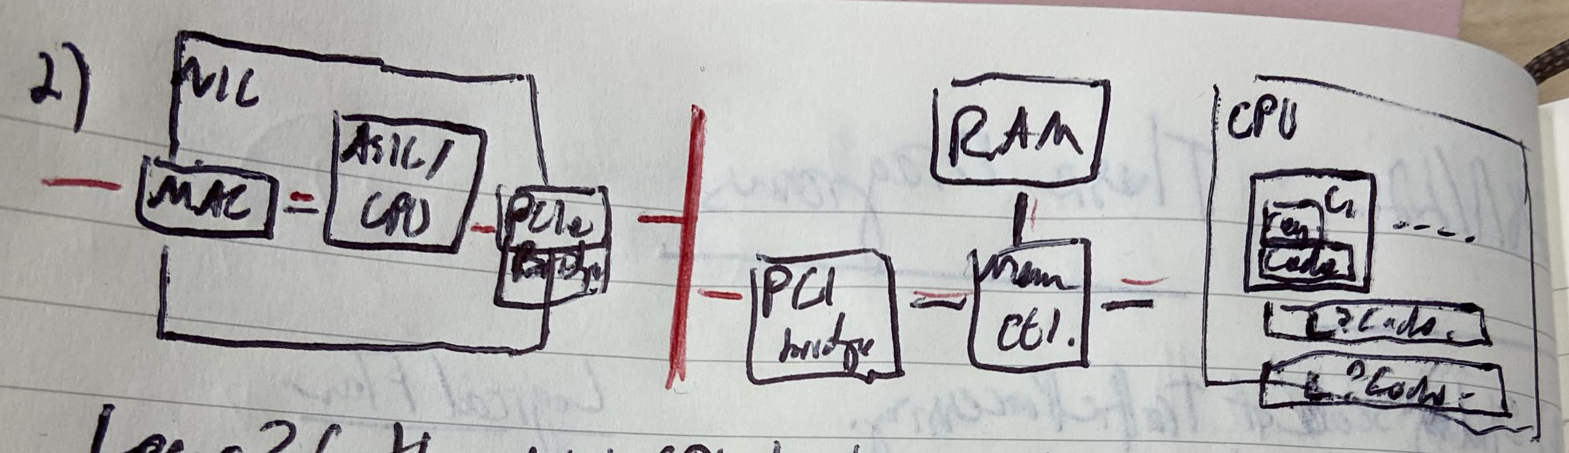
\includegraphics{diagrams/pdp-lit/pci-draft}}
	\resizebox{\linewidth}{!}{\colorlet{pci-nic}{uofgforest}
\colorlet{pci-nic-inner}{white}
\colorlet{pci-cpu}{uofglavendar}
\colorlet{pci-cpu-inner}{white}
\colorlet{pci-subcpu}{pci-cpu!20}

\colorlet{pci-conn}{black}
\colorlet{pci-pcie}{uofgrust}
\colorlet{pci-pktpath}{uofgcobalt}

\begin{tikzpicture}
	\node at (0,0) (nic-box) {};
	\draw[color=pci-nic,fill=pci-nic!10] (nic-box) rectangle ++(5,-2);
	\node at ($(nic-box) + (0.5,-0.3)$) {\gls{acr:nic}};

	\draw[color=black,fill=pci-nic-inner!10] ($(nic-box) - (1,1.75)$) rectangle ++(2,1) node[pos=.5] (mac) {\gls{acr:mac}};
	\draw[color=black,fill=pci-nic-inner!10] ($(mac) + (1.5,-0.5)$) rectangle ++(2,1) node[pos=.5,align=center] (asic) {\gls{acr:asic}/\\\gls{acr:cpu}};
	\draw[color=black,fill=pci-nic-inner!10] ($(asic) + (1.5,-0.5)$) rectangle ++(2,1) node[pos=.5,align=center] (nic-pci) {\gls{acr:pcie}\\Bridge};

	\draw[color=black,fill=pci-nic-inner!10] ($(nic-pci) + (2.5,-1.5)$) rectangle ++(2,1) node[pos=.5,align=center] (ram-pci) {\gls{acr:pcie}\\Bridge};
	\draw[color=black,fill=pci-nic-inner!10] ($(ram-pci) + (1.5,-0.5)$) rectangle ++(2,1) node[pos=.5,align=center] (mem-ctl) {Memory\\Controller};
	\draw[color=black,fill=pci-nic-inner!10] ($(mem-ctl) + (-1,1)$) rectangle ++(2,1) node[pos=.5,align=center] (ram) {\gls{acr:ram}};

	\node at ($(nic-box) + (12.5,0)$) (cpu-box) {};
	\draw[color=pci-cpu,fill=pci-cpu!30] (cpu-box) rectangle ++(4,-3);
	\node at ($(cpu-box) + (0.5,-0.3)$) {\gls{acr:cpu}};

	\begin{scope}[on background layer]
		\draw[color=pci-cpu,fill=pci-cpu!10] ($(cpu-box) + (0.25, 0.25)$) rectangle ++(4,-3);
		\draw[color=pci-cpu,fill=pci-cpu!20] ($(cpu-box) + (0.125, 0.125)$) rectangle ++(4,-3);
	\end{scope}

	\draw[color=black,fill=pci-nic-inner!10] ($(cpu-box) + (0.5,-2.75)$) rectangle ++(3,0.75) node[pos=.5,align=center] (l3) {L3 Cache};

	\node at ($(cpu-box) + (0.5,-0.5)$) (subcpu-box) {};
	\draw[color=pci-cpu,fill=pci-subcpu!30] (subcpu-box) rectangle ++(2,-1.25);
	\node at ($(subcpu-box) + (0.75,-0.3)$) {Core 1};

	\draw[color=black,fill=pci-nic-inner!10] ($(subcpu-box) + (0.125,-1.15)$) rectangle ++(1.75,0.55) node[pos=.5,align=center] (l1-l2) {\small{}L1/L2};

	\node[text=black] at ($(subcpu-box)+(2.7,-0.75)$) {\huge$\cdots$};

	% pci-cpu

	\node at ($(nic-pci) + (1.75, 1.5)$) (pcie-top) {};
	\node at ($(pcie-top) - (0, 3.5)$) (pcie-bot) {};
	\draw[very thick, color=pci-pcie] (pcie-top) -- (pcie-bot);
	\draw[very thick, color=pci-pcie] ($(pcie-top) - (0,1.5)$) -- (nic-pci);
	\draw[very thick, color=pci-pcie] ($(pcie-top) - (0,2.5)$) -- (ram-pci);

	\node[text=pci-pcie] at ($(pcie-top)+(0,0.1)$) {\glslink{acr:pcie}{\color{pci-pcie}PCIe}};

	% --------------

	\draw[transform canvas={yshift=-1.5pt}, color=pci-conn, very thick] (mac) -- (asic);
	\draw[transform canvas={yshift=-1.5pt}, color=pci-conn, very thick] (asic) -- (nic-pci);

	\draw[transform canvas={yshift=-1.5pt}, color=pci-conn, very thick] (ram-pci) -- (mem-ctl);
	\draw[transform canvas={xshift=-1.5pt}, color=pci-conn, very thick] (mem-ctl) -- (ram);
	\draw[transform canvas={yshift=-1.5pt}, color=pci-conn, very thick] (mem-ctl.east) -- ($(mem-ctl.east) + (1,0)$);

	\draw[color=pci-pktpath, very thick] (mac.west) -- ($(mac.west) - (1,0)$);
	\draw[transform canvas={yshift=1.5pt}, color=pci-pktpath, very thick] (mac) -- (asic);
	\draw[transform canvas={yshift=1.5pt}, color=pci-pktpath, very thick] (asic) -- (nic-pci);

	\draw[transform canvas={yshift=1.5pt}, color=pci-pktpath, very thick] (ram-pci) -- (mem-ctl);
	\draw[transform canvas={xshift=1.5pt}, color=pci-pktpath, very thick] (mem-ctl) -- (ram);
	\draw[transform canvas={yshift=1.5pt}, color=pci-pktpath, very thick] (mem-ctl.east) -- ($(mem-ctl.east) + (1,0)$);

	\draw[transform canvas={yshift=3pt}, color=pci-pktpath, very thick] (nic-pci) -| ++(1.85,0) |- (ram-pci);
\end{tikzpicture}}
	\caption[A simplified view of the physical packet path on host machines.]{A simplified view of the physical packet path on host machines, shown {\color{pci-pktpath} in blue}. Moving packets between the \gls{acr:nic} and \gls{acr:cpu} is more involved than simple steering, as packets must be moved across the \gls{acr:pcie} bus and \gls{acr:dma}'d into host memory. The host \gls{acr:cpu} is made aware of packet arrivals by either \glspl{acr:irq} or polling ring buffers in memory which the \gls{acr:nic} writes into. This introduces additional latency, even when the networking stack supports direct insertion into the \gls{acr:cpu} cache. Note that this figure leaves aside \gls{acr:numa} constraints and costs arising from having several \glspl{acr:cpu}.}\label{fig:pdp-lit-pci}
\end{figure}

Most of the impact on traffic processing originates also from logical costs due to the \gls{acr:os}'s device and network stack management.
\Cref{fig:pdp-lit-offloading} lays out some of these stages in the Linux environment.
Primarily, the \gls{acr:os} kernel is notified that packet \glspl{acr:dma} have completed via \glspl{acr:irq}, at which point a kernel thread is awoken and the device driver is called to transfer the packet contents into a \gls{acr:skb} usable by the stack.\sidenote{The conventional network stack does not poll for packets. While this would reduce any additional delays associated with the interrupt model, running a device driver in a busy loop is not generally considered feasible or acceptable. This model \emph{does} drive specialist frameworks like \gls{acr:dpdk}, which we'll cover, but this requires care and significant changes in userland code.}
Awaking a thread does not guarantee that it will be instantly ready to serve the packet, adding latency, while readying packet \glspl{acr:skb} adds additional per-packet overheads which harm receive-side latency and throughput.
The Linux network stack itself must then inspect \glspl{acr:skb} to handle decapsulation, transport logic such as \gls{acr:tcp} and \gls{acr:cca} management, and connection handling---among other functions related in more much detail by existing work~\parencite{DBLP:conf/sigcomm/CaiCVH021}.
Finally, the packet is served over a socket to a (possibly sleeping) userland thread, who may require a context switch before the received data may be finally used---again, another source of processing latency.

%?? IRQs enable, but can take time for CPU to awaken.
%?? Linux network stack -- encapsulations, segmentation, \gls{acr:tcp} and transport logic, connection management etc.
%?? typical sockets: sleep rather than poll (and again, await context switch).

Interestingly, these additional hardware and software costs are analogous to route-level steering on a smaller scale.
%?? Make the argument around existing doftware needing a reasonable OS?
A more specialised packet processing stack might be one way to remove many of the software costs, but such a clean-slate proposition would lock packet processing programs out of access to software reliant on typical \gls{acr:os} functionality.
%Instead, recent years have brought greater kernel support for eliminating as many of these stages as possible.
\emph{Host offloading frameworks} aim instead to reduce this steering as far as possible with support from the \gls{acr:os} or hardware; either by eliminating much of the logical packet processing invoked by the \gls{acr:os} kernel, or moving user code to an earlier point in the stack.
Returning to \cref{fig:pdp-lit-offloading}, we now focus on the user-programmable blocks.
In the best case, SmartNIC hardware allows user code to be moved onto the \gls{acr:nic} completely, removing \gls{acr:pcie} bus transfer latency as packet processing no longer needs to touch the \gls{acr:cpu}.
Of course SmartNICs are typically less capable than hosts (in clock speeds and included \glspl{acr:fu}), and for that reason we'll briefly discuss kernel bypass methods such as \gls{acr:dpdk} and offloads enabled by \gls{acr:ebpf}.
As before, offloaded user code may be some or all of a larger program, potentially divided into fast and slow paths according to whether host compute is needed.


%?? \cref{fig:pdp-lit-pci} phys, \cref{fig:pdp-lit-offloading} logical.
%
%?? Include representative numbers for e.g. PCIe and so on.
%
%?? \gls{acr:pcie}~\parencite{DBLP:conf/sigcomm/NeugebauerAZAL018}
%
%?? \gls{acr:ram}
%
%?? Host stack~\parencite{DBLP:conf/sigcomm/CaiCVH021}
%
%?? Intel DDIO~\parencite{intel-ddio} -- L3 Cache
%
%?? Mention \gls{acr:dma} somehow.

%?? Offloading to SmartNIC good at eliding \gls{acr:pcie} costs.

\begin{figure}
	%	\resizebox{\linewidth}{!}{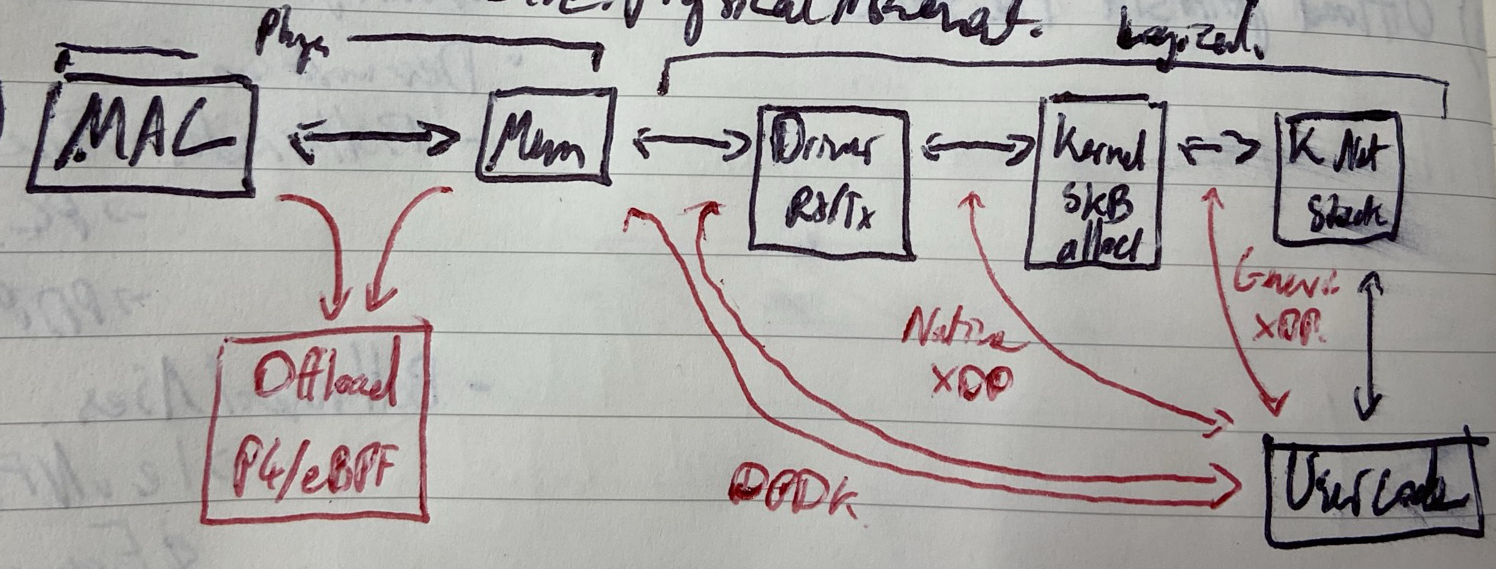
\includegraphics{diagrams/pdp-lit/offloading-draft}}
	\resizebox{\linewidth}{!}{\colorlet{ol-phys}{uofgforest}
\colorlet{ol-log}{uofglavendar}
\colorlet{ol-user}{uofgrust}
\colorlet{ol-userland}{ol-user!75}

\colorlet{ol-arrow}{black}
\colorlet{ol-user-arrow}{ol-user}

\begin{tikzpicture}
	\draw[color=ol-phys,fill=ol-phys!10] (0,0) rectangle ++(2,1) node[pos=.5] (mac) {\gls{acr:mac}};
	\draw[color=ol-phys,fill=ol-phys!10] ($(mac) + (2, -0.5)$) rectangle ++(2,1) node[pos=.5] (nic) {\gls{acr:nic}};
	\draw[color=ol-phys,fill=ol-phys!10,align=center,text=black] ($(nic) + (2, -0.5)$) rectangle ++(2,1) node[pos=.5] (mem) {Memory\\\& Cache};

	\draw[color=ol-log,fill=ol-log!10,align=center,text=black] ($(mem) + (2, -0.5)$) rectangle ++(2,1) node[pos=.5] (rx-tx) {Driver\\Rx/Tx};
	\draw[color=ol-log,fill=ol-log!10,align=center,text=black] ($(rx-tx) + (-1, -2.5)$) rectangle ++(2,1) node[pos=.5] (skb) {Kernel\\\gls{acr:skb} Alloc};
	\draw[color=ol-log,fill=ol-log!10,align=center,text=black] ($(skb) + (-1, -2.5)$) rectangle ++(2,1) node[pos=.5] (ns) {Network\\Stack};

	\draw[color=ol-userland, fill=ol-userland,align=center, text=white, rounded corners] ($(ns) + (-5, -0.5)$) rectangle ++(2,1) node[pos=.5] (userland) {Userland\\Code};

	\draw[color=ol-user, fill=ol-user,align=center,text=white, rounded corners] ($(nic) + (-2, -3.5)$) rectangle ++(2,1) node[pos=.5] (smartnic-offload) {Offload\\C/P4/\glslink{acr:ebpf}{\color{white}eBPF}};

	\draw[color=ol-user, fill=ol-user,align=center,text=white, rounded corners] ($(skb) + (-5, -0.5)$) rectangle ++(2,1) node[pos=.5] (xdp-offload) {Offload\\\glslink{acr:ebpf}{\color{white}eBPF} (\glslink{acr:xdp}{\color{white}XDP})};

	% --------

	\node[color=ol-phys] at (0.75, 1.35) {\large{}Physical};
	\node[color=ol-log, rotate=270] at (11.5, 0.5) {\large{}Logical};

	% --------

	\draw[<->, thick, color=ol-arrow] (mac) -- (nic);
	\draw[<->, thick, color=ol-arrow] (nic) -- (mem);
	\draw[<->, thick, color=ol-arrow] (mem) -- (rx-tx) node[midway, above] {\small{}\glspl{acr:irq}};
	\draw[<->, thick, color=ol-arrow] (rx-tx) -- (skb);
	\draw[<->, thick, color=ol-arrow] (skb) -- (ns);


	\draw[<->, thick, color=ol-user-arrow, shorten >=0.25cm,shorten <=0.3cm] (ns) -- (userland) node[midway, below] {\small{}Socket};
	\draw[<->, thick, color=ol-user-arrow, shorten >=0.12cm,shorten <=0.17cm] (nic) -- (smartnic-offload) node[midway, left, align=center] {\small{}SmartNIC\\Offload};
	\draw[<->, thick, color=ol-user-arrow, shorten >=0.12cm,shorten <=0.12cm] (rx-tx) -- (xdp-offload) node[midway, above, sloped] {\small{}Native \glslink{acr:xdp}{\color{ol-user-arrow}XDP}};
	\draw[<->, thick, color=ol-user-arrow, shorten >=0.05cm,shorten <=0.12cm] (skb) -- (xdp-offload) node[midway, above] {\small{}Generic \glslink{acr:xdp}{\color{ol-user-arrow}XDP}};
	\draw[<->, thick, color=ol-user-arrow, shorten >=0.12cm,shorten <=0.12cm] (userland) -- (xdp-offload) node[midway, right] {\small{}\texttt{AF\_XDP}};

	\draw[<->, thick, color=ol-user-arrow, shorten >=0.12cm,shorten <=0.12cm, out=200,in=150] (mem) to node[left] {\small{}\glslink{acr:dpdk}{\color{ol-user-arrow}DPDK}} (userland);
\end{tikzpicture}}
	\caption[The logical packet processing stack on host machines, and how the DPDK and XDP frameworks interface with it and user code.]{The logical packet processing stack on host machines, and how the \gls{acr:dpdk} and \gls{acr:xdp} frameworks interface with it and user code. Rounded, filled boxes represent user code. Offload frameworks are useful because they either allow \gls{acr:os} kernel code to be bypassed altogether (\gls{acr:dpdk}), or for packet modification and transmission to be pushed further down the stack (\gls{acr:xdp}). Offloaded \gls{acr:ebpf} user code may typically pass packets to the network stack after some amount of processing, send packets directly back to the \gls{acr:nic} for transmission, or pass packets to user code using a zero-copy mechanism such as \texttt{AF\_XDP}. Crucially, all these mechanisms excise various amounts of processing or imprecise waiting for  interrupts, reducing latencies and increasing packet processing throughput. More details on the logical portion of the stack are presented by \Textcite{DBLP:conf/sigcomm/CaiCVH021}.}\label{fig:pdp-lit-offloading}
\end{figure}

\paragraph{Early optimised network stacks}
Although less relevant in today's landscape, we'll discuss here some older frameworks offering varying degrees of network stack bypass for completeness.
%?? First: what does each do.
\texttt{PF\_RING}~\parencite{pf-ring} was motivated by changes in the kernel to prevent \gls{acr:irq} livelock at high speeds, which helped but were insufficient to achieve line rate processing at the receiver.
It created a kernel-user ring buffer per socket, where received packets are copied into all ring buffers with remaining space allocated to the \gls{acr:nic}, bypassing the network stack.
\emph{Netmap}~\parencite{DBLP:conf/usenix/Rizzo12} made use of shared kernel and user memory over ring buffers to place userland code between the \gls{acr:nic} driver and the host networking stack for a given interface.
I.e., a packet bound from the \gls{acr:nic} to the network stack would traverse kernel$\rightarrow$user$\rightarrow$kernel.
It offered specific innovations in copy elimination, batching of syscalls, and effective preallocation of packet buffers and metadata versus \gls{acr:skb}-based packet buffer management.
Specifically, netmap's rings contain memory descriptors which point into a shared buffer, as compared with \texttt{PF\_RING}'s explicit byte buffers (which must be copied into).

\paragraph{Kernel bypass}
In constrast to the above, Intel's \glsxtrfull{acr:dpdk}~\parencite{dpdk,dpdk-ad-paper} bypasses the kernel entirely, by running \gls{acr:nic} drivers in userland.
\glspl{acr:nic} are run via poll-mode drivers in \gls{acr:dpdk}'s \emph{environment abstraction layer}, which manages core mappings to receive and transmit queues, memory allocation and device operation.
%?? In constrast to the above, runs NIC in userland using poll-mode drivers.
User programs interface with the abstraction layer to receive packets using a poll-only model, which results of course in consistently high (or maxed out) \gls{acr:cpu} utilisation.
In exchange for this trade-off, programs designed to receive and process packets from \gls{acr:dpdk} entirely bypass the kernel, greatly reducing per-packet overhead.
Since packets must be received from \gls{acr:dpdk}'s abstraction layer, user programs must be rewritten to account for the poll-based semantic model and vastly different buffer lifetime semantics versus the traditional stack---e.g., correct handling and disposing of ring buffer descriptors.
This can be worked around to some extent by efficient user-space \emph{library kernel} \gls{acr:os} implementations of the traditional Linux networking stack~\parencite{DBLP:conf/eurosys/ThalheimUPBP21}.
%?? Mention that this can be used to drive library OS impls of the standard net stack if so needed.~\parencite{DBLP:conf/eurosys/ThalheimUPBP21}

\paragraph{eBPF and XDP}
The \glsxtrfull{acr:ebpf}~\parencite{ebpf-history} is a register-based \gls{acr:risc} \gls{acr:vm} and assembly language.
Owing to its simple and easily-implemented design, \gls{acr:ebpf} is used today for moving packet programs early into the kernel, instrumenting standard kernel functions using tracepoints, and offloading.
\gls{acr:ebpf} is derived from the earlier \emph{BSD Packet Filter}~\parencite{DBLP:conf/usenix/McCanneJ93}, which was a two-register \gls{acr:vm} designed to allow user-written programs to be safely executed at the kernel level---in this case, to prevent unnecessary packet copies for unwanted traffic or packet contents in monitoring applications like \emph{tcpdump}.
`Arbitrary, sandboxed user code in the kernel' was certainly an idea with potential, and in light of its wider uptake \gls{acr:ebpf} was modified to become more capable and closer in architecture to modern \glspl{acr:cpu}: for instance ten \qty{64}{\bit} registers, atomic instructions, maps, and function call opcodes to make use of functions exposed by the kernel.

Today the \gls{acr:vm} abstraction enables fast and safe execution of such programs by \gls{acr:jit} compilation and verification, and is now well-suited for offloading to SmartNICs and similar devices.
Making this more accessible, industry-standard compilers support \gls{acr:ebpf} as a compile target from languages such as C and Rust.
%\gls{acr:ebpf} is now a compiler target for simple platform-agnostic programs, which are well-suited for offloading due to their bounded size, verifiable semantics, and the simplicity of the underlying \gls{acr:vm}. ?? ebabling JIT?
In the Linux \gls{acr:os} kernel, \gls{acr:ebpf} programs may be triggered by \emph{hooks} for instrumenting its operation via \emph{kprobes} and \emph{tracepoints}---a program specifies its type with respect to its intended hook, from which the kernel knows which functions an \gls{acr:ebpf} program may call (effectively enforcing an \gls{acr:api}).
Programs are accepted if and only if they are loop-free, terminate, have bounded size, and simulated bounds checks on array accesses are well-defined.
Larger programs may be constructed by building chains of tail calls between these smaller \gls{acr:ebpf} blocks.
Userland and \gls{acr:ebpf} programs communicate using \emph{maps}, which are a generic abstraction around containers such as arrays, hash tables, and longest-prefix match tables which may be concurrently read and modified by user and kernel code.

%\gls{acr:ebpf}~\parencite{ebpf-history}, 
%?? It should be clear that \gls{acr:ebpf}'s role in the network owes an inestimable debt to \emph{smart packets}.

%?? Came from BPF~\parencite{DBLP:conf/usenix/McCanneJ93}

%?? eBPF also allows exec of user code at various points in kernel for instrumentation etc. via \emph{kprobes} and \emph{tracepoints}.

Linux's \glsxtrfull{acr:xdp}~\parencite{DBLP:conf/conext/Hoiland-Jorgensen18} uses \gls{acr:ebpf} to place user-specified code into the packet processing path.
Naturally, these programs undergo the same verification and \gls{acr:jit} compilation as traditional \gls{acr:ebpf} hook programs, and run one instance per \gls{acr:nic} receive queue.\sidenote{This can present a bottleneck for the amount of code offloaded to this stage in \glspl{acr:nic} without support for several receive queues---the \gls{acr:xdp} hook must meet strict timing constraints. \qty{1}{\giga\bit\per\second} integrated \glspl{acr:nic} present this problem, in my experience.}
\gls{acr:xdp} hook programs have a slightly more privileged role, and are called before the network stack for each packet arriving on an interface to determine its ultimate fate.
For instance, packets may be modified and immediately transmitted back on the wire, dropped, passed on to the remainder of the host networking stack, or redirected to another \gls{acr:xdp} program or user-land socket.
Consider once more \cref{fig:pdp-lit-offloading}.
If driver support is offered, offloaded code may be run before any \gls{acr:skb} management or creation with zero memory copies (\emph{Native}).
Otherwise, the program runs after \gls{acr:skb} creation (\emph{Generic}), but before any part of the remainder of the networking stack.
Note that packets may be served \emph{entirely} in the \gls{acr:xdp} hook by making use of maps, packet modification, and the \texttt{XDP\_TX} immediate transmit action, minimising latencies as far as possible in an \gls{acr:irq}-based system.
Moreover, \gls{acr:xdp} is flexible enough to fit into a wide variety of packet processing stacks.

This is accompanied by the \texttt{AF\_XDP}~\parencite{lwn-af-xdp} socket family, which may circumvent the remainder of the network stack by sending the packet directly to user code from an \gls{acr:xdp} hook.
As a notable application, the main packet path of the \gls{acr:ovs} software switch has been migrated to \texttt{AF\_XDP} due to its performance and ease of injecting user code into the kernel stack~\parencite{DBLP:conf/sigcomm/TuWAP21}.
The file descriptors of these sockets are placed in an \gls{acr:ebpf} map, enabling faster packet processing by reducing the time delta between the fast and slow packet paths.
User and kernel code share a set of ring buffers, queues, and a large block of preallocated UMEM to pass packet-sized buffers between another in response to completions and demand, a mechanism that is outwardly similar to netmap.
While map sizes are fixed at compile time, sockets have a many-to-one relationship with the actual hook program, enabling per-core or per-application service of packets to make better use of cache coherence.
\texttt{AF\_XDP} sockets support both poll- and \gls{acr:irq}-mode at the user level.

%?? Umem lmao

\paragraph{Experimentally demonstrating latency benefits}
%?? Quick description of the experimental setup.
%?? Maybe plot and run through the experimentes I'm doing atm?
We can illustrate the relative performance of these frameworks against one another (and the traditional \texttt{AF\_PACKET}) using a simple microbenchmark.
We can measure approximately how much time each `cut' into the kernel saves by connecting two identical machines together over a single link (using \gls{acr:nic} hardware with support for these technologies).
One machine generates and timestamps traffic, while the other performs a \gls{acr:mac} swap function using the intended framework to return packets to the first machine to measure sampled \glspl{acr:rtt}.

To do so, the two commodity host machines (\emph{Src} and \emph{Swap}) were set up using an Intel Core i7-4790 (\qtyproduct[product-units=single]{4 x 3.6}{\giga\hertz}), \qty{16}{\gibi\byte} \gls{acr:ram} (DDR3, \qty{1866}{\mega\hertz}), an Intel X710 40GbE \gls{acr:nic}, running Ubuntu 21.10 (5.13.0-30-generic).
The hardware lacks support for direct cache access functions like Intel DDIO, and clock scaling was disabled for predictable measurement.
The machines were connected over a \qty{40}{\giga\bit\per\second} direct copper cable using a single Rx/Tx queue on \emph{Swap}.
Traffic was generated on \emph{Src} using Pktgen-\gls{acr:dpdk}~\parencite{pktgen-dpdk} to generate \qty{64}{\byte} packets at \qty{1}{\giga\bit\per\second}, timing \num{20000} packets per framework using the included uniform latency sampler.
\emph{Swap} was configured in four ways, using \gls{acr:dpdk}'s \emph{testpmd} application for receipt and forwarding:
\begin{description}
	\item[\gls{acr:dpdk}] \emph{testpmd} was set to swap \gls{acr:mac} addresses and forward packets, using the X710 \gls{acr:nic}'s \texttt{i40e} poll-mode driver.
	\item[Native \gls{acr:xdp}] A custom \gls{acr:ebpf} program set to swap packet \gls{acr:mac} addresses and always return \texttt{XDP\_TX} was manually installed.
	\item[\emph{\texttt{AF\_XDP}}] \emph{testpmd} was set only to forward packets, using the \gls{acr:xdp} poll-mode driver with a custom \gls{acr:ebpf} program to swap \gls{acr:mac} addresses before redirecting to the first supplied \gls{acr:xdp} socket. This driver makes use of polling support for \texttt{AF\_XDP} sockets.
	\item[\emph{\texttt{AF\_PACKET}}] \emph{testpmd} was set to swap \gls{acr:mac} addresses and forward packets, using the \texttt{AF\_PACKET} poll-mode driver.
\end{description}
\gls{acr:ebpf} programs were written in Rust (version 1.59.0) using an in-development version of the redbpf framework.
Note that in the \texttt{AF\_XDP} case the choice to perform \gls{acr:mac} swapping in the \gls{acr:xdp} hook (rather than userland) is deliberate, to measure the time taken to reach user code after service by the offloaded \gls{acr:ebpf} program.

\begin{figure}
	\centering
	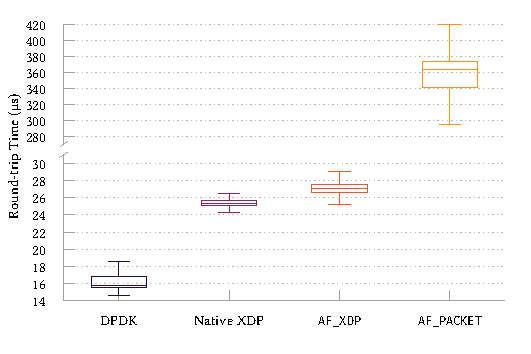
\includegraphics[keepaspectratio,width=\linewidth]{plots/xdp/macswap-rtts-split}
	\caption[A microbenchmark of bypass/offload frameworks' effects on packet RTTs.]{A microbenchmark of bypass and offload frameworks' effects on packet \glspl{acr:rtt}. In line with our expectations from the amount of processing removed by each framework according to \cref{fig:pdp-lit-offloading}, \emph{\gls{acr:dpdk}} adds the lowest base latency, followed by \emph{Native \gls{acr:xdp}} and \texttt{AF\_XDP}. All of these achieve significantly better forwarding latencies than na\"{i}ve use of \texttt{AF\_PACKET}.\label{fig:xdp-microbench}}
\end{figure}

%?? Testpmd on send-side
%
%?? Transmission relies on the PMD.
%?? in XDP, macswap function is handled by the \gls{acr:ebpf} program installed at the xdp hook. Else, PMD.

%Intel Core i7-4790 (\qtyproduct[product-units=single]{4 x 3.6}{\giga\hertz}), \qty{16}{\gibi\byte} RAM (DDR3, \qty{1866}{\mega\hertz}), 1~\texttimes{} Intel X710 40GbE NIC, Ubuntu 21.10 (5.13.0-30-generic)

%?? two machines as above, no DDIO or other direct-cache access, single rx queue

%?? clock scaling disabled

%?? Pktgen-\gls{acr:dpdk}~\parencite{pktgen-dpdk}, \qty{64}{\byte} packets at 

%?? macswap function: done in \gls{acr:xdp} hook where possible. use DPDK to do so with the device-specific poll-mode driver (\emph{DPDK}), and emulated drivers (\texttt{AF\_XDP} and \texttt{AF\_PACKET}).

\Cref{fig:xdp-microbench} shows a clear performance hierarchy between the offload and bypass frameworks: \emph{\gls{acr:dpdk}} has a \qty{11401}{\nano\second} lower median \gls{acr:rtt} than offloaded \gls{acr:ebpf} code, which in turn is \qty{2167}{\nano\second} lower than \texttt{AF\_XDP}.
Distributions of latencies fall within a tight bound of \qtyrange{3}{5}{\micro\second}, with \emph{Native \gls{acr:xdp}}'s \glspl{acr:rtt} appearing less varied than \texttt{AF\_XDP}---it's difficult to make any conclusive observations here due to variability in the send and receive stacks of both machines.
The inclusion of \texttt{AF\_PACKET} is, to some extent, a strawman.
It does however demonstrate quite succinctly the absolute worst-case behaviour of not making use of kernel or stack bypass technologies for generic packet processing---order-of-magnitude worse latencies and tail behaviour.
It's worthwhile to remind ourselves that \gls{acr:xdp} hook code can run alongside the standard Linux networking stack, benefiting applications without needing to reconsider and rewrite their socket handling code.
Additionally, by swapping testpmd for a Rust-based receive stack and reading from the \texttt{AF\_XDP} socket (using blocking I/O rather than polling), early measurements saw a \qtyrange{39}{50}{\micro\second} gap between \gls{acr:ebpf} and userland code.

%?? Extra lat and very high variability, comparatively.

\subsection{Frameworks for automatic offloading}\label{sec:frameworks-for-automatic-offloading}
One of the strengths of the above offload technologies is that their architects are keen to see them achieve widespread adoption, and as such they tend to be well-integrated with existing technical stacks.
For instance, \gls{acr:ebpf} has been offered as a codegen target for both the LLVM and GCC compiler suites since 2015 and 2019 respectively~\parencite{ebpf-llvm,ebpf-gcc}, enabling code written in popular high-level languages like C or Rust to be compiled to this level.
This presents an interesting research challenge: adapting these developments towards lower-level fragments of such programs intelligently, such that offloading can improve performance with little input from the programmer.
I provide here a brief overview of the higher- and lower-level tooling developed by the research community to either lower the barrier for adoption (and easily migrate existing \gls{acr:nf} solutions), or to improve on the potential performance benefits.

\paragraph{Host-to-SmartNIC}
\emph{Floem}~\parencite{DBLP:conf/osdi/PhothilimthanaL18} presents a \gls{acr:dsl} in Python for Click-like dataflow programming to be offloaded, specifying a processing graph of logical blocks which compiles to C code for hosts and target NICs.
Users specify which parts of the processing graph execute on each offload device, making this a useful (but not necessarily optimal) tool for investigating offloading strategies.
Per-packet metadata is user-specified, but the compiler can infer which state must cross \gls{acr:cpu}-to-\gls{acr:nic} boundaries with the aid of annotations.
Individual blocks (and the centralised queue handling) require user implementation in C for each target device class.

\emph{iPipe}~\parencite{DBLP:conf/sigcomm/LiuCSKPG19} runs C language programs on SmartNICs and hosts according to whether traffic is at risk of suffering from SmartNIC resource contention.
Although iPipe aims to maximise the amount of traffic served by the SmartNIC, processing is dynamically `unoffloaded' back to the host machine if the SmartNIC's monitored load is too great (i.e., if packet latencies increase).
In contrast to Floem, iPipe uses an actor programming model to allow for more dynamic control flow between program blocks; this runtime `unoffloading' and migration occurs at actor-level granularity.
iPipe assumes identical language support between the host and offload target. 
While C language support is common, identical semantics aren't guaranteed depending on how tailored the target SmartNIC requires code to be.
The design is effective enough to protect underlying traffic while achieving improved latency and throughput bounds over a similar \gls{acr:dpdk} dataplane.

\emph{Gallium}~\parencite{DBLP:conf/sigcomm/ZhangZK20} converts C++ Click programs to automatically leverage \gls{acr:pdp} resources between several segments---pre- and post-host offloaded P4 segments, sandwiching a single host C++ program.
This model gives greater flexibility than C-based offloading by enabling program division between, say, a Tofino switch and its attached controller \gls{acr:cpu}, however this imposes greater restrictions on what logic may be offloaded.
Gallium uses LLVM \gls{acr:ir} to determine read-write dependencies between variables and basic-blocks of the packet processing chain's control flow graph, and account for \gls{acr:pdp} hardware's capabilities around packet reads (i.e., \gls{acr:pdp} datapaths typically can't access packet bodies past $\sim$\qty{300}{\byte}).\sidenote{SmartNICs do not have such limitations, so this is mainly a consideration for \gls{acr:psa} switches or more general deployment. Such access is still limited to \texttt{extern}s, and may need to retrieve packet data from larger, slower blocks of \gls{acr:ram}.}
By annotating these blocks based on their ordering requirements and offload capability, as well as limiting metadata movement to under \qty{100}{\byte}, they generate the desired program splits by maximising the \gls{acr:ir} instructions moved into P4 code---ideally identifying fast paths if there exist cases where the host part can be elided.
This approach successfully achieved higher throughput and lower latency than a purely host-based FastClick solution for trojan detection.
The main drawback is that Gallium requires some annotation to translate Click primitives into \glspl{acr:mat} as well as read or write dependencies on function parameters, otherwise the conversion to P4 minimises the additional work per target device.

\paragraph{eBPF in the network}
As a solution to OpenFlow's limited action set, \emph{BPFabric}~\parencite{DBLP:conf/ancs/JouetP17} proposed that \gls{acr:ebpf} programs should be used in place of explicit \gls{acr:mat} definitions.
%?? well-suited because \gls{acr:ebpf} simple, non-Turing, bounded exec time suited for real-time.
\gls{acr:ebpf} was seen as well-suited here because of its simple semantics and restrictions which kept it non-Turing complete; thus, having bounded execution times suitable for real-time packet processing.
Its authors keep most of the OpenFlow machinery intact---the device-controller relationship specifically---but instead install one \gls{acr:ebpf} program per device, encoding its entire view of the dataplane.
\gls{acr:mat} layouts and program needs are included in the ELF metadata of supplied \gls{acr:ebpf} programs, and the return value of such a program is the desired output port (including special OpenFlow-style ports to forward packets to the controller).
Such programs would be compiled to from a constrained, high-level, C-like language with the typical \gls{acr:ebpf} restrictions on loops, with a device-local loader playing the role of the Linux kernel's verifier.
%?? device-local loader plays the role of kernel in verification etc.
%?? Keeps all the relevant OpenFlow machinery
%?? One program per device, which returns the output port for a given packet (incl special outputs like controller, etc.).
%?? MAT layout in the ELF header.
%?? Forward-thinking: maps enables and accounts for switch/nic-local updates to table state without controller.
The proposal contains one particularly forward-thinking aspect---\gls{acr:ebpf} maps would be mutable from within the target device, enabling and accounting for switch- or \gls{acr:nic}-local updates to table state without the aid of a controller.
It did not, however, solve the problem of how SmartNICs or other target devices should actually implement the required \gls{acr:ebpf} execution engines.

\emph{hXDP}~\parencite{DBLP:conf/osdi/BrunellaBBPSBCP20} designs a dedicated \gls{acr:cpu} on \gls{acr:fpga} hardware tailored for \gls{acr:ebpf} program execution on network traffic.
Given that hXDP is tailored towards running unported \gls{acr:xdp} programs, this coprocessor is augmented with dedicated support for helper functions and memory for maps.
Their model iteratively runs an expanded \gls{acr:ebpf} \gls{acr:isa} rather than converting programs into a complete pipelined circuit to offer faster redesign and reinstall times: complete circuit planning takes a long time, while \gls{acr:jit} compiling an \gls{acr:ebpf} program into their new \gls{acr:isa} is relatively quick.
Additionally, their compiler tracks functional dependencies to encode the program in \gls{acr:vliw} form to maximise hardware parallelism, while also applying network-specific optimisations.
%This includes some very cool details on around VLIW instruction-level parallelism built into their ISA and figured out during compile-time.
This dedicated design outperforms hosts and \gls{acr:nfp} SmartNICs in latency, but typically exhibits worse throughput due to its slower single core.

%?? andimpl maps, kernel functions

%?? offers a concrete solution to this problem

\paragraph{eBPF in hosts}
Preliminary work has been proposed on automatically splitting \gls{acr:ebpf} programs between an \gls{acr:xdp} part and userland part~\parencite{DBLP:conf/conext/ShahinfarMSSBA21}.
This approach considers both horizontal splits, i.e., subdividing code into \gls{acr:ebpf} chunks using tail-calls, and vertical user$\leftrightarrow$kernel splits of code.
%I think their XDP vs.~AF\_XDP split test confirms that the first handler in the XDP hook is basically single-threaded, which probably has some implications for our use of it as an offload.
This appears to have promise for increasing application throughput, although optimal splitting points vary based on the use case.

\emph{Morpheus}~\parencite{DBLP:conf/asplos/MianoSRRA22} offers a more sophisticated form of \gls{acr:jit} compilation for \gls{acr:ebpf} and \gls{acr:dpdk} programs---using lightweight sketch-based measurement to drive profile-guided optimisation and recompilation on a regular time interval.
This produces compiled bytecode tailored to the observed traffic distribution, twinned with inlining of tables into fast and slow paths dependent on \gls{acr:mat} contents.
While most of this optimisation is provided as-standard when working with profiled LLVM \gls{acr:ir}, Morpheus provides compiler plugins to account for key features such as \gls{acr:mat} logic and match classes.
%?? sketch-based profiling (`adaptive measurement')
%?? adaptive inlining based on \gls{acr:mat} contents, fast and slow paths
%?? guards around maps to gate de-optimisation
\gls{acr:ebpf} programs use guard mechanisms to fall back to deoptimised program code as required (\gls{acr:mat} or profile changes), while userland code is broken into smaller optimised chunks that are be atomically updated via a trampoline function.
%?? programs broken down into smaller chunks: map indirection for tailcalls in ebpf, trampolines in user for atomic update
Morpheus achieves substantial latency and throughput improvements on larger dataplane programs such as Katran~\parencite{katran}, in spite of the additional overhead of adaptive trace monitoring.

\paragraph{FPGAs and the wider network}
%?? mention how it came to this: this was an alternate solution to latency or throughput concerns which plague VNF approaches as they scale (see Metron~\parencite{DBLP:conf/nsdi/KatsikasBKSM18} paper for good discussion of RSS, etc., which solve these problems in their own way)

\emph{ClickNP}~\parencite{DBLP:conf/sigcomm/LiTLPLXXC16} presents an approach for migrating entire Click processing graphs to NetFPGA devices.
While tools to convert C programs into the required VHDL specifications exist, the authors find that they lead to suboptimal code in area and \gls{acr:lut} usage.
As is standard in Click-like approaches, functions are written as directed graphs of predefined Click-like blocks, in this case each specifically written in a hardware description language to achieve lower \gls{acr:fpga} resource utilisation.

\emph{Metron}~\parencite{DBLP:conf/nsdi/KatsikasBKSM18} builds on OpenBox to break \gls{acr:vnf} chains into stateless and stateful logic: stateless processing is offloaded to the network via the ONOS controller (making use of heterogeneous OpenFlow and P4 hardware), while function chains are dynamically allocated one per core.
%?? weak \gls{acr:mat} programmability of modern \glspl{acr:nic} to control core steering.
Crucially, the performance of these stateful functions is maximised by using the weak \gls{acr:mat} programmability of modern \glspl{acr:nic} to control core steering dynamically (and consistently) according to load and to balance traffic across replicated functions.
Chains are allocated in the network using a combination of topology and current load information (preferring local processing).

\emph{Flightplan}~\parencite{DBLP:conf/nsdi/SultanaSGPHSBDL21} splits a P4 program into subchunks, placed and routed between heterogeneous \gls{acr:pdp} hardware along a path---\glspl{acr:fpga}, hosts, servers, \glspl{acr:npu}, and \glspl{acr:asic}---for pipelining (i.e., performance) or redundancy.
Flightplan's compiler breaks its input dataplane's \gls{acr:ir} into blocks according to user annotations in the supplied P4 code.
Further user-given annotations denote manual implementations of specific \texttt{extern}s, to enable device-specific acceleration of key functions such as compression or error correction.
Their disaggregation procedure inserts logic before and after splits to handle metadata and state passing.
These blocks are statically analysed to extract the data dependencies between sub-functions, which are then composed into a chain over the routing infrastructure using a set of program, resource, and network rules.

%\paragraph{Misc P4 translations.}
%T4P4S~\parencite{DBLP:conf/hpsr/VorosHKLTL18} converts P4 programs into C, which are linked against a target-specific network hardware abstraction layer.
%This seems to be the most effective host deployment for P4 at the moment, since it buys you DPDK-capable P4 dataplane installation compared to how terribly slow BMv2 is known to be.
%Slower than native DPDK, but outpaces OvS, and allows definition of HAL binaries in SmartNIC C code as needed too.
%
%$\mu$P4~\parencite{DBLP:conf/sigcomm/SoniR0DF20} extends P4C to decompose parser and action code into independent subprograms, to simplify porting behaviours between different switch models (V1Model, PSA, SUME, ...).
%
%Lyra~\parencite{DBLP:conf/sigcomm/GaoZLMZTSCZY20} is a language for running Network Programming Language friendly programs (i.e., same constraints as P4 programs) across heterogeneous switch hardware, plus placement constraints.
%
%?? P4 Verification~\parencite{DBLP:conf/sigcomm/TianGLZCZDYMTLW21}---also shows use of \gls{acr:pdp} switches in real large-scale networks (\gls{acr:isp}?)

\section{In-network compute use cases}\label{sec:in-network-compute-use-cases}
%?? Lead-in, describe...
To make the value of \glspl{acr:pdp} and in-network compute clearer, I present here a selection of specific applications that have been improved or enabled outright by these new capabilities.
These include advances in network monitoring and telemetry, application acceleration by in-network services, and how the network may allow improved or more dynamic transport and routing.
Finally, as it is of particular importance to this thesis and the overall goal of \gls{acr:ddn}, we shall examine in close detail \gls{acr:ml}-related use cases.
It must be said that the works shown here are indicative, rather then exhaustive.
Interested readers should also examine dedicated surveys such as that of \Textcite{DBLP:journals/access/KfouryCB21}.

\subsection{Network monitoring}\label{sec:network-monitoring}
%?? The P4 ecosystem already presents novel, openly-available, fine-grained traffic measurement techniques that can be installed and controlled with ease~\parencite{DBLP:conf/sigcomm/GuptaHCFRW18,DBLP:conf/sigcomm/ChenFKRR18,DBLP:conf/sosr/GhasemiBR17}
%?? Maybe explain them?
Traffic monitoring solutions built on non-\gls{acr:pdp} fabrics can be imprecise or limited.
Routers typically provide sampled data such as sFlow, Netflow, or IPFIX, along with imprecise timing at the \unit{\micro\second} and \unit{\milli\second}-level~\parencite{rfc7011,rfc3954}.
While this offers useful insight at the aggregate or per-flow level, fine temporal or transient dynamics are lost, such as queue states or per-packet arrival timestamps which might help identify bursty flows or the culprits of microbursts on the network.
Precision is not the sole culprit here, \unit{\micro\second}-level per-packet data simply has too much volume in both raw bytes and packets to meaningfully export beyond the device.
\gls{acr:pdp} fabrics offer here new ways to gather, aggregate, and process per-packet, -device, and -port state in-situ.

%and observe... from
%Acquiring \unit{\nano\second}
%?? Per-packet, \unit{\nano\second}- or \unit{\micro\second}-level data
%?? too much to export. (eve though us level in current tools)
%?? device- and port-local state


%However, flow classification solutions today can usually only rely on sampled data provided by routers, such as sFlow, Netflow, or IPFIX, along with imprecise timing (\si{\micro\second} and \si{\milli\second}-level)~\parencite{rfc7011,rfc3954}.
%While sampled, low-precision telemetry can be used to classify network traffic based on some flow properties (such as port and protocol numbers)~\parencite{DBLP:conf/iwcmc/RossiV10}, it cannot be used to classify based on fine temporal properties (\eg, identifying bursty flows and senders that can cause microbursts and buffer overflow on the network).

\emph{Sonata}~\parencite{DBLP:conf/sigcomm/GuptaHCFRW18} splits dataflow queries on packet streams between \gls{acr:pdp} hardware and Apache Spark-based collector host machines.
These dataflow queries are described in the usual functional style (maps, filters, etc.)---Sonata aims to maximise processing and data reduction performed by the dataplane to ease the burden on stream processing host machines.
This includes \gls{acr:ilp}-based dynamic query refinement to filter out unneeded packets as early as possible.
\emph{Snappy}~\parencite{DBLP:conf/sigcomm/ChenFKRR18} detects microbursts---transient spikes in queue occupancy leading to packet loss---by maintaining sketches to estimate the queue occupancy of long flows.
The input data, packet arrival and departure events, are naturally too numerous to track externally, numbering in the millions or billions of packets per second at switch scale.
Long flows dominating output port queues are determined as the root cause of these events, and such heavy-hitter flows may be marked, dropped, re-routed, or rate-limited as required.
\emph{Dapper}~\parencite{DBLP:conf/sosr/GhasemiBR17} implements in-depth, per-flow analysis of \gls{acr:tcp} traffic in pure P4.
When required, Dapper follows lightweight measurement of per-flow byte counts and timestamping with more in-depth estimation of congestion and receive window sizes, host reaction times, and latencies to determine whether the sender, network, or receiver is the true bottleneck (without inspecting state on either end-host machine).

A particularly noteworthy family of measurement techniques associated with \glspl{acr:pdp} is \glsxtrfull{acr:int}~\parencite{p4-int}.
\gls{acr:int} allows for network state---including formerly inaccessible state such as egress queue/buffer occupancies and traversed paths---to be collected and reported without control plane intervention.
To do so, packets contain header fields marking `telemetry instructions' to be executed by participating devices along their path.
Typically, requested measurement data is appended to (or written into a dedicated space in) an \gls{acr:int} header attached to the packet, piggybacking onto existing traffic, thus keeping packet arrival rates fairly constant.
\gls{acr:int} sinks then strip this auxiliary data from packets, collect it, and report it to the control plane; enabling finer-grained measurement of network state in routes as well as network-assisted \glspl{acr:cca} and load balancing schemes.
%?? typically, by piggybacking.
To some extent, this is a specialisation of \emph{tiny packet programs}~\parencite{DBLP:conf/sigcomm/JeyakumarAGKM14}, which aimed to enable the same end goals and applications by taking a somewhat `active networking'-like tack---including simple load and push instructions for switch values inside every packet.
Instead, \gls{acr:int} focusses on collecting pre-defined metadata such as node and port IDs, buffer states, and link utilisations.
These fine-grained measurements can be added per-hop, also enabling packet paths to be traced without contacting the control plane as required by \emph{NetSight}'s postcarding~\parencite{DBLP:conf/nsdi/HandigolHJMM14}.
At the same time, these collected measurements allow operators to build a full-network picture of per-hop latencies, utilisations, and buffer states.
%?? INT use-cases~\parencite{DBLP:conf/sigcomm/JeyakumarAGKM14}, postcards~\parencite{DBLP:conf/nsdi/HandigolHJMM14}
While powerful, \gls{acr:int} is expensive to deploy.
Although extra per-packet overhead can be bounded for some operations, \gls{acr:int}'s typical hop-by-hop recording causes a linear growth in packet sizes according to path length.
Network \glspl{acr:mtu} limit the amount of per-packet state which can be added for larger packets.
To combat these difficulties, \emph{PINT}~\parencite{DBLP:conf/sigcomm/BasatRLAYM20} introduces aggregation and approximation mechanisms to bound per-query values below a certain budget of bits.
Most notably, per-hop data collection is uniformly randomly divided over a packet's path, combined with numerical approximations and the use of sketches for per-flow state on switches themselves.
\emph{INT-label}~\parencite{DBLP:conf/infocom/Song0JC00L21} aims to reduce redundant measurements and curtail adverse effects on flows by attaching a labelling interval to every port, which can be adaptively altered to account for losses.
This includes a probabilistic component such that packets with \gls{acr:int} labels are more likely to receive and carry additional metadata (shielding most packets from the costs of \gls{acr:int}).
\emph{LightGuardian}~\parencite{DBLP:conf/nsdi/ZhaoYLYCLZWWWZ21} reduces the impact of exporting per-flow sketches by dividing them into \emph{sketchlets} over several packets, to be reconstructed by \gls{acr:int} sink nodes.

\gls{acr:pdp} hardware also offers a toolkit for the diagnosis and mitigation of more specific network problems.
By using \gls{acr:int}-like switch tracking, \emph{Unroller}~\parencite{DBLP:conf/conext/0004BKAYM20} detects persistent routing loops.
Unlike \gls{acr:int}, Unroller tracks only the minimum ID seen by a packet, periodically overriding this at geometrically increasing intervals.
To detect \gls{acr:ddos} attack victims in pure P4, \emph{INDDoS}~\parencite{DBLP:journals/tnsm/DingSPCS21} uses count-min sketches to estimate the number of flows inbound for a given server.
\emph{Jaqen}~\parencite{DBLP:conf/uss/LiuNNLK0BYS21} offers a framework for \gls{acr:pdp}-augmented \gls{acr:isp} networks to detect and mitigate many volumetric, amplification, and semantic \gls{acr:ddos} attacks (though not \glspl{acr:lfa}).
To gather state, it maintains sketches of source/destination \gls{acr:ip} addresses and ports alongside counters, as well as useful primitives like native stateless P4 implementations of \texttt{SYN} cookie functions and approximate Bloom filter allow- and block-lists.
State is polled by the control plane, which interprets sketches to perform higher-level logic (e.g., observing thresholds, significant changes) and installs detection and mitigation functions using a heuristic algorithm to ensure sufficient coverage.

\subsection{Service acceleration and offloading}\label{sec:ddn-service-accel}
Distributed data structures, such as key-value stores, are a foundational part of many data centre applications for process coordination and concurrency control.
\emph{NetChain}~\parencite{DBLP:conf/nsdi/JinLZFLSKS18} and \emph{FLAIR}~\parencite{DBLP:conf/nsdi/TakruriKAA20} offer P4-based implementations of distributed key-value stores, routing and serving requests and updates subject to a chain replication protocol for reliability, achieving an order-of-magnitude latency improvement for reads and writes.
NetChain in particular uses a mixture of \glspl{acr:mat} and registers to accelerate index lookups and store data respectively, though both eliminate steering costs and host stack costs.
As another example, distributed hash tables like \emph{No-hop}~\parencite{DBLP:conf/ancs/HugerichSS21} see improved lookup times from route caching enabled by the \gls{acr:pdp} ecosystem.

%?? Enabling services
Other advances built on \gls{acr:pdp} infrastructure have made it easier for network administrators to scale their infrastructure up to account for additional hosts, handling the associated routing, load balancing, and subscription at lower cost than prior methods.
Facebook's open-source \emph{Katran} L4 load balancer~\parencite{katran,katran-blog} makes use of \gls{acr:xdp} to co-exist on existing service nodes, offer low-disruption updates, and presents lower latency than userland solutions.
No performance numbers are shared, though it is reportedly used aggressively in production.
\emph{Cheetah}~\parencite{DBLP:conf/nsdi/BarbetteTYKMPC20} implements consistent load balancing for arbitrary functions at switch scale on Tofino hardware, where it achieves strong tail performance guarantees for flows even during active churn.
An intriguing use of \gls{acr:pdp} hardware that has been presented is how it may allow \emph{packet subscriptions}~\parencite{DBLP:conf/conext/JepsenFMFCS20}---networks may offer an accelerated, Apache Kafka-style publish-subscribe architecture.
This includes higher-level tooling to synthesise a complex, content-driven dataplane at runtime (including broadcast, replication and routing).

There have also been key advances in using \gls{acr:pdp} hardware for stream processing and fusion to accelerate management and monitoring as well as application-level use-cases---including some realisation of the earlier discussion on protocol boosters.
\emph{DAIET}~\parencite{DBLP:conf/cloud/SapioACK17} proposes performing the \emph{aggregate} step of \emph{partition-aggregate} workloads (i.e., MapReduce) by organising workers and programmable switches into processing trees.
\Textcite{DBLP:conf/conext/HypoliteSHDDS20} investigate how to make good use of (\gls{acr:npu}-type) SmartNIC parallelism to perform \gls{acr:dpi} and payload matching tasks through \emph{DeepMatch}.
By making good use of the \gls{acr:nfp}'s parallelism and memory models, they offer fast, flow reorder-aware processing by the Aho-Corasick algorithm.
\emph{\textsc{Bolt}}~\parencite{DBLP:conf/infocom/WangZLLLJX21} then implements Aho-Corasick on Tofino switches using \glspl{acr:mat}---however, this requires full recirculations to extract a fixed size byte slice per pass.
To reduce traffic impact on infrastructure while freeing host resources, \emph{ZipLine}~\parencite{DBLP:conf/conext/VaucherYFLS20} uses packet checksum functionality on Tofino switches to implement transparent traffic compression.

%?? In-network storage/caching~\parencite{DBLP:conf/eurosys/SchmidPWEP20}

\subsection{Transports, protocols, and routing}\label{sec:pdp-uses-transports}
Making better use of networks through \gls{acr:te}, more sophisticated \glspl{acr:cca}, and more adaptive routing is a challenging but worthwhile endeavour.
\gls{acr:pdp} hardware allows us to place more complex decisions and new algorithms at a lower level, where they can take advantage of the fine-grained or complex state and measurements that in-network compute gives us access to (\cref{sec:network-monitoring}).
Our ideal aims are that flows would converge to their optimal fair-share of bandwidth faster (and with greater accuracy), better respond to congestion and incast events, or more dynamically make use of network capacity.
Moreover, it allows us to consider new schemes for doing so as networked use cases change or evolve over the years to come.
We'll consider here some ways in which \gls{acr:pdp} hardware makes the management and operation of networks faster or more resilient by measurement, cooperation, or novel algorithms.

%?? ROuting and load balancing (over paths) more dynamic, fairer and more uniform than e.g. \gls{acr:ecmp}
Multipath networks are commonly used to achieve high bisection bandwidth between hosts, but require specialised schemes like \gls{acr:ecmp} to balance load across their fabric.
\gls{acr:pdp} hardware is configurable enough to allow the development and deployment of new routing protocols which are more dynamic, fairer, and uniform; ideally, with less control plane interaction.
\emph{HULA routing}~\parencite{DBLP:conf/sosr/KattaHKSR16} provides a P4-based solution targeting data centre networks, using periodic broadcast probes sent in-band to update every switch's estimate of its best path to every other destination.
\emph{Contra}~\parencite{DBLP:conf/nsdi/HsuBCRW20} extends this with a custom policy language to encode constraints and more involved routing criteria (i.e., to support arbitrary topologies): probes also obey these rules in the reverse path.
Both approaches achieve substantial improvements to fairness above \gls{acr:ecmp}, and scale well by tracking only a single cost per destination.

\gls{acr:aqm} allows for flow and packet priorities to be expressed for their egress from a switch, enabling shaping or \gls{acr:te} to ensure optimal \gls{acr:qos} or \gls{acr:qoe}---for instance, prioritising the packets of short flows (minimising the risk they are dropped by a full buffer) to minimise relative \glspl{acr:fct}.
\emph{\gls{acr:pifo}}~\parencite{DBLP:conf/sigcomm/SivaramanSACCAB16} queues allow for individual packet priorities and dispatch times to be determined by the ingress pipeline of a \gls{acr:pdp} switch's \glspl{acr:mat}---offering almost arbitrary programmability---but require this dedicated hardware primitive.
\emph{PIEO}~\parencite{DBLP:conf/sigcomm/Shrivastav19} queues extend their expressiveness further by allowing arbitrary elements to be dequeued, also.
However, the reality is that commodity P4-based switches aren't yet suitable for enabling many of the \gls{acr:aqm} disciplines developed by the research community.
\Textcite{DBLP:conf/im/KunzeGSWR21} find that \gls{acr:aqm} solutions must be co-designed for the target environment, for instance pipeline and register access constraints make it impossible to express some algorithms.
Implementation of \gls{acr:aqm} schemes like \emph{PIE}~\parencite{rfc8033} is found to require numerous tradeoffs, with meaningful performance costs in each case.

\glspl{acr:cca} play a key role in ensuring that congestion-aware transport protocols are able to make use of their maximal fair share of bandwidth in the network.
Original \emph{and} state-of-the-art \glspl{acr:cca} in use on the wider Internet, such as \gls{acr:tcp} BBR~\parencite{DBLP:journals/queue/CardwellCGYJ16}, operate on minimal information transfer between hosts or endpoints, and are often reliant on congestion \emph{signals} from the network like packet losses and changes to \glspl{acr:rtt}.
This is a necessity to minimise the network costs of transferring state, to co-exist with heterogeneous \glspl{acr:cca}, and to isolate their logic from the network itself to prevent wider ossification.
This has significant drawbacks.
Advanced, control-theoretic \glspl{acr:cca} like the \emph{PCC} family of \glspl{acr:cca}~\parencite{DBLP:conf/nsdi/DongLZGS15,DBLP:conf/nsdi/DongMZAGGS18} or \emph{Copa}~\parencite{DBLP:conf/nsdi/ArunB18} are computationally expensive compared to their forebears.
Having more, high-quality information also prevents fairness issues which may arise from needing to rely on carefully tuned responses to otherwise opaque signals from the network, such as BBRv1's noted unfairness with other \gls{acr:tcp} traffic~\parencite{DBLP:conf/imc/WareMSS19}.
%?? BBR~\parencite{DBLP:journals/queue/CardwellCGYJ16} is unfair~\parencite{DBLP:conf/imc/WareMSS19}
%?? cost of logic and importance of good information to make decisions on.
Even older \glspl{acr:sdn} show the value of high-quality, global information---consider \emph{OTCP}~\parencite{DBLP:conf/noms/JouetPP16}, which calculates optimal pairwise \gls{acr:tcp} parameters by using OpenFlow and its supporting protocols to actively measure static network characteristics like latencies and link bandwidths.
\gls{acr:pdp} infrastructure can go further still, and offers new ways to offload \gls{acr:cca} logic or to augment it with assistance from the network.
Data centre networks are best placed for this---\emph{NDP}~\parencite{DBLP:conf/sigcomm/HandleyRAV0AW17} is a receiver-driven \gls{acr:cca} where P4 switches truncate packet payloads when buffers are at risk of exhaustion, while senders choose network routes for fairer load balancing.
Header-only packets are prioritised, providing a dedicated fast path for control packets and effective congestion signals.
\emph{HPCC}~\parencite{DBLP:conf/sigcomm/LiMLZFTCZKAY19} instead uses the \gls{acr:int} techniques discussed above to expose path characteristics and loads to a connection's sender.
\texttt{ACK} messages carry their packet's \gls{acr:int} data; the sender adjusts its target rate per-\texttt{ACK} (minor) and per-window (major).
As this specifically accelerates remote \gls{acr:dma}, endpoints require \gls{acr:fpga}-enabled \glspl{acr:nic}.
To enable offload of arbitrary \gls{acr:cca} logic, \Textcite{DBLP:conf/nsdi/ArashlooLGRWW20} present \emph{Tonic} as a framework for expressing the \emph{transport logic} (what data segments are sent at what times) while handling connection and buffer management.
These may be modified via small user-programmable blocks containing \glspl{acr:alu} with access to per-flow state.
The remainder of their framework handles (de)packetisation, packet transmission for many waiting flows, and \gls{acr:dma} handling.
%?? Hi~\parencite{DBLP:conf/nsdi/ArashlooLGRWW20} Network stacks being moved into NICs to reduce latency/CPU utilisation, mainly for datacentre use-cases---otherwise, \SI{100}{\giga\bit\per\second} can't be hit. New API \emph{Tonic} for transport layer in user code (send, data management), DMA to NIC and let it handle all (de)packetisation. ``Transport logic'' goes to Tonic. Main design is datacentres, so not very high BDPs (long-fat) $\rightarrow$ \si{\kilo\byte} inflight data.

\subsection{Machine learning}\label{sec:inc-uses-pdp-ml}
\gls{acr:pdp} hardware and in-network compute give us the capabilities to perform packet and flow classification (\emph{inference}) at line rate, and to accelerate data centre-scale \emph{training} of \gls{acr:ml} models for both \gls{acr:ddn} and other domains.
As we'll examine throughout \cref{chap:ddn}, \gls{acr:ml} techniques make it possible to learn and act upon complex patterns or relationships in network data to perform all manner of management and optimisation tasks more effectively.
While I cover specific implications of data formats and training algorithms later (\cref{sec:numerical-representations-for-embedded-ml,sec:learning-an-approximation}), the gist is that machine learning inference and training are generally dependent on floating point data (as training gradients are real-valued), peripheral accelerators like \glspl{acr:gpu} or \glspl{acr:tpu}, and are computationally complex.
%?? Using ML needs putting at accel (slow)
Host machines are, then, in many ways the best-suited location for \gls{acr:ml} training and inference at scale, but these come at the cost of network and \gls{acr:pcie} costs to reach the host's \gls{acr:cpu}, and then further data transfer costs over \gls{acr:pcie} to the \gls{acr:gpu}.
Inference at the host thus presents real tradeoffs: either choose throughput by batching queries and new data for the \gls{acr:gpu}, or choose consistent (tail) latencies by using the \gls{acr:cpu}.
This becomes all the more interesting and challenging when we consider the additional classes and finer granularity of measurement data exposed by \gls{acr:pdp} hardware, such as those discussed earlier in \cref{sec:network-monitoring}.
%?? Exporting the kinds of telemetry of interest in \cref{sec:network-monitoring} is infeasible, but if we can act on it...
Of course, use case depending, this raw data is produced at volumes and rates far too high to meaningfully move across the network.
Host machines can't handle raw packet-per-second demands at this scale, let alone when every packet must undergo some \gls{acr:ml} algorithm.
Per-packet inference (i.e., for security, \gls{acr:qos}, or \gls{acr:te} classification) is thus untenable in this framework.
Ideally we would process this in \gls{acr:pdp} devices, but this is at odds with their resource-limited nature---limited \gls{acr:alu} capabilities, a definite lack of floating-point hardware, and small amounts ($\mathcal{O}\left(\text{\unit{\kibi\byte}--\unit{\mebi\byte}}\right)$) of high-speed memory.
This leaves us with a difficult dilemma.
%?? training  and inference costs
%?? batching, etc.
In-network \gls{acr:ml} research aims to solve this (preferably at line-rate) by focussing on the modifications needed to install inference techniques onto \gls{acr:pdp} hardware---tailoring algorithms and data formats to the target device.
%: more details on suitable data representations are presented through \Cref{sec:fixed-point-and-binary}.

\paragraph{Inference}
%?? ML in the dataplane~\parencite{DBLP:conf/hotnets/XiongZ19,DBLP:conf/sigcomm/SanvitoSB18,DBLP:journals/corr/abs-1801-05731,DBLP:journals/corr/abs-2009-02353,langlet-ml-netronome,DBLP:journals/corr/abs-2002-08987}
\emph{IIsy}~\parencite{DBLP:conf/hotnets/XiongZ19} investigates per-packet inference using pre-trained classical \gls{acr:ml} models on programmable switch hardware, as well as methods for cheaply updating models at runtime through the control plane.
In particular they use custom parsers as a feature extraction mechanism, and convert parameters and inference logic into \glspl{acr:mat} to implement these models using pure P4.
This guarantees their compatibility with the vast majority of \gls{acr:pdp} devices in deployment.
These include multiple implementations of \glspl{acr:svm}, decision trees, Na\"{i}ve Bayes, and K-means classifiers, executing but not training on these devices.
In particular, they investigate the best use of tables in these scenarios---per-feature, per-class and per-cluster---noting that all cases exhibit different impact from quantisation and processing length (in recirculations).
%Evaluating using the P4$\rightarrow$NetFPGA workflow~\cite{DBLP:conf/fpga/IbanezBMZ19} against an IoT traffic classification (and QoS assignment) problem, even in the best cases (decision trees, SVMs, K-means) a feature/class limit of \num{20} is suggested.
%This suggests that training (or adaptive policy modification in RL's case) are relatively unexplored---but potentially costly, given that these cannot be implemented using only table matches.

\glspl{acr:nn} require more specific considerations due to their variable structure, but their implementation in \gls{acr:pdp} hardware is an important topic due to their ubiquity in \gls{acr:ml} and \gls{acr:ddn} research.
\textcite{langlet-ml-netronome} has shown the viability of \gls{acr:nn} inference using \qty{64}{\bit} quantisation on \gls{acr:nfp} SmartNICs, but this can observe high ($\sim$\qty{500}{\micro\second}) inference latency on line rate traffic for larger inputs.
This compute model has the main downside, however, of being unsuited to \gls{acr:rmt} or \gls{acr:psa} switches.
\glspl{acr:bnn} have been shown to be a promising data format for \gls{acr:pdp} hardware; not least because they are computationally efficient, but because they admit ready conversion to \glspl{acr:mat}, and are thus suitable for deployment on \emph{all} P4 devices.
\emph{BaNaNa SPLIT} shows how these \glspl{acr:bnn}, installed in \glspl{acr:nic}, can as a partial offload mechanism~\parencite{DBLP:conf/sigcomm/SanvitoSB18}; \gls{acr:dnn} inference is often carried out on the \gls{acr:cpu} to remove latencies imposed by \gls{acr:gpu} batching and transfer, but they show that the fully-connected layers of such networks can be accelerated further by \glspl{acr:nic} subject to some accuracy loss.
\emph{N2Net}~\parencite{DBLP:journals/corr/abs-1801-05731} and \emph{N3IC}~\parencite{DBLP:journals/corr/abs-2009-02353} examine, collectively, different ways of running \glspl{acr:bnn} among SmartNICs, P4 implementations, and \glspl{acr:fpga} to achieve line-rate, in-path, per-packet inference of classes for use by later tables or packet tagging.

\emph{Taurus}, examined earlier in \cref{sec:frontiers-in-programmable-networks}, allows for implementation of the inference mechanisms above closer to line-rate without needing to substantially alter input and policy data formats.
At fabrication time, Taurus may be configured to use the required fixed-point depth.
Other specialised hardware includes \emph{BrainWave}~\parencite{DBLP:conf/isca/FowersOPMLLAHAG18}---an \gls{acr:npu} designed solely for parallelised \gls{acr:simd} \gls{acr:nn} inference---which reduces batching by \qty{32}{\texttimes} compared to \gls{acr:gpu} acceleration.
However, inference still requires $\mathcal{O}{\left(\text{\si{\milli\second}}\right)}$ in representative use cases~\parencite{Duarte2019}.
%Even novel \gls{acr:dma} techniques such as \emph{GPUDirect}~\parencite{gpudirect} halve but do not eliminate \gls{acr:pcie} transfers.
%?? A recent line of research in the community has been to investigate \emph{Binarised/Bitwise Neural Networks} (BNNs)~\parencite{DBLP:conf/nips/HubaraCSEB16,DBLP:journals/corr/KimS16,DBLP:journals/corr/MiyashitaLM16} for line-rate packet classification.
%?? \emph{BaNaNa SPLIT} shows this as an offload mechanism~\parencite{DBLP:conf/sigcomm/SanvitoSB18,DBLP:journals/corr/abs-1801-05731}; DNN inference is often carried out on the \emph{CPU} to reduce latency imposed by GPU batching and transfer, but fully-connected layers can be accelerated further by NICs.
Neither, however, allows for on-device training; Taurus instead sends sampled data to the controller, while similar provisions could apply to a BrainWave installation.

\paragraph{Training}
On \gls{acr:ml} training, most research on how \gls{acr:pdp} hardware may be applied falls into the optimisation of \emph{distributed \gls{acr:ml} training} via in-network aggregation.
The main use case here involves many nodes in a network exchanging gradient vectors to be combined with a shared model---however, latency-optimal schemes based on central \glspl{acr:ps} have strongly synchronised inbound traffic which causes high, bursty losses and significant bandwidth consumption near the traffic destination.
Aggregating these gradients is simply vector addition, which any interim node may perform to reduce the upstream traffic burden.
\gls{acr:pdp} hardware provides a sound basis for the kinds creative co-design needed to ensure optimal training behaviour here, making better use of the network \emph{and} improving final training times and performance.
%\Cref{sec:distributed-training} covers the surrounding context and solutions in more detail.
At a high-level, \emph{iSwitch}~\parencite{DBLP:conf/isca/LiLYCSH19} uses the plasticity of \gls{acr:fpga} devices to implement a dedicated floating-point adder and gradient storage; gradient packets are signalled to the dataplane using a reserved pool 2 \gls{acr:dscp}~\parencite{rfc2474} value, triggering their aggregation (and eventual retransmission to the \gls{acr:ps}).
Solutions targeting general \gls{acr:pdp} switches---e.g., \emph{ATP}~\parencite{DBLP:conf/nsdi/LaoLMCWAS21} and \emph{SwitchML}~\parencite{DBLP:conf/nsdi/SapioC0NKKKMPR21}---instead must rely on fixed-point data formats to enable this in these environments.
%\emph{iSwitch}~\parencite{DBLP:conf/isca/LiLYCSH19} uses NetFPGA-SUME hardware to implement special handling for RL model update packets, building floating-point adders and limited storage space into bump-in-the-wire \glspl{acr:nic} to achieve \qtyrange{3.66}{3.71}{\times} faster training.
%\emph{SwitchML}~\parencite{DBLP:conf/nsdi/SapioC0NKKKMPR21} converts a programmable \gls{acr:tor} switch \emph{into a \gls{acr:ps}}, offering this as a P4 program built on fixed-point quantisation.
%\emph{ATP}~\parencite{DBLP:conf/nsdi/LaoLMCWAS21} extends this to a best-effort service and custom transport protocol in front of the true \gls{acr:ps}, falling back to floating point on detection of overflows and offering better support for several dynamic jobs.
Unfortunately, to the best of my knowledge true on-device model training for \gls{acr:pdp} \gls{acr:ml} or \gls{acr:rl} hasn't yet been examined beyond the work I present in \cref{chap:in-net-rl}.
%The closest I have seen in the literature is Taursu, but even then...

%\section{Hardware Designs}
%
%?? Mention FPGA vs many-core
%
%?? P4 etc. can actually all run on commodity hardware, which offers a third (suboptimal) hardware class.
%
%?? Ref the paper that Haruna presented \parencite{DBLP:conf/icc/MafiolettikDMRV20}: pareto front of work-division optimality for SmartNICs (i.e., addition of high-latency cores).
%
%?? How do these limit and influence what code can be run on different device classes? The time taken to adapt the network?
%
%\subsection{Models of Parallelism}
%
%\subsection{Flexibility}
%
%\subsection{Mapping Software Frameworks}

%\section{Operation and Management}
%
%?? network-network comms? BGP
%
%?? IGP?
%
%?? packets routed on a per-hop basis from their perspective: may be higher level in practice (MPLS, path switching within a gateway)
%
%?? How can we examine this? High-level (above), mid-level ()
%
%?? Two axes: end-to-end protocol and fabric behaviour. interact in a very delicate way (i.e., host )
%
%?? named-data networking as potential structure of the Internet?~\parencite{DBLP:journals/ccr/0001ABJcCPWZ14}
%?? Can I use this to suggest/outline problems which might be solved/encountered in a future Internet?
%
%?? Talk about \gls{acr:as} families here: \glspl{acr:isp}, hypergiants~\parencite{DBLP:conf/sigcomm/GigisCMNKDKS21}...
%?? Data centres: refer to e.g. google Espresso [sigcomm 2017] as big SDN deployments, Jupiter, recent paper too?

%\subsection{Fixed-Function Hardware}
%
%\subsection{Software-Defined Networking}
%
%?? Run through the historical context. Why? What led into P4 (OpenFlow, network operating systems...)
%
%?? \gls{acr:ovs}~\parencite{DBLP:conf/nsdi/PfaffPKJZRGWSSA15} huge here.
%
%?? A survey to mine for stuff~\parencite{DBLP:journals/comsur/NunesMNOT14}
%
%?? Tie into PDP here: active networking and TPP . Think about the concept of protocol boosters~\parencite{DBLP:journals/jsac/FeldmeierMSBMR98}. (NOT READ)

%\section{Traffic Characteristics}
%
%\subsection{Evolution}
%
%\subsection{Emerging Protocols}
%
%\subsection{Limitations}

\section{Summary}\label{sec:pdp-summary}
%Eh.
%
%?? History
%
%This chapter begins by motivating and describing initial attempts at dataplane programmability in the '90s (primarily \emph{active networking}), how control-plane programmability and \gls{acr:sdn} arose in their wake, and the reasons behind these movements' respective failures and successes (\cref{sec:from-fixed-function-to-fully-programmable}).
%\Cref{sec:modern-pdps} introduces modern, programmable dataplanes by tracing efforts parallel to \gls{acr:sdn} for improving the performance of host-based packet processing such as \glspl{acr:vnf}, before leading into the emergence of specialised \gls{acr:pdp} hardware and its legacy owed to \gls{acr:sdn} and \glspl{acr:npu}.
%This is followed by commentary on how the original active networking movement differs from modern \glspl{acr:pdp} (and context behind the latter's successful adoption), as well as a selection of open challenges and proposals in \gls{acr:pdp} programming languages and hardware designs.
%\Cref{sec:offloading-and-in-network-compute} then provides the rationale for \emph{offloading} service logic to \gls{acr:pdp} hardware and within host network stacks, and describes existing research on using these capabilities to automatically accelerate existing dataplane programs.
%To further motivate in-network compute, point solutions which take advantage of the execution environment and more granular view of network data to improve measurement and operation are described (\cref{sec:in-network-compute-use-cases}).
%Finally, \cref{sec:problems-in-modern-networks} provides some literature on volumetric \gls{acr:ddos} attacks (and defences against them) as necessary background for \cref{chap:ddos-rl}.

I have described the history of programmable networks from their initial forays to-date, including what is now a rich tapestry of software-defined routing and bespoke programmable devices mixed with heavily-optimised host machines.
We've examined how advances in dataplane programmability enable application performance to be meaningfully improved---lower latencies and higher throughputs---by taking clever advantage of \gls{acr:pdp} hardware.
In particular, this covers the importance of moving high-performance services to the right execution environment---\emph{offloading}.
Most crucially, considering in-network compute from the outset enables a plethora of ways to meaningfully improve the management of today's networks.
%Finally, we covered a large-scale problem in modern networks---the ever-present threat of \gls{acr:ddos} attacks---and how Internet traffic characteristics make its solution more difficult.

My concluding thought is that \gls{acr:pdp} and its use cases present a vibrant, ongoing line of research---particularly when we consider how it can be combined with \gls{acr:ddn}.
It offers today a source of raw device data which we would have never been able to feasibly use or export, as well as the necessary tools to perform complex data analysis at line-rate and switches' scale.
At the same time it provides ways of helping host machines scale further via aggregation, and a promising location to perform complex, data-driven logic and reaction.
I am of the opinion, however, that it is still a field in its adolescence.
The hardware solutions and designs which have arisen and entered widespread market adoption (e.g., \gls{acr:rmt}$\rightarrow$Tofino) are impressive, powerful and capable---but they are the first wave of fully programmable devices at this scale and this form-factor, and we should expect even more innovation in hardware and languages as the field evolves.
This may well take the form of incoming heterogeneity, as device manufacturers produce \gls{acr:pdp} devices tailored to different use cases in much the same vein as \emph{Taurus}.
Projects like \emph{BrainWave} reiterate that network hypergiants already hold the means and motivation to do just this.